\chapter{Integração de uma Arquitetura de Transporte QUIC sobre ICE}
\label{chap:implementation}

Este capítulo descreve o desenvolvimento da comunicação entre \textit{peers} atrás de um NAT através das técnicas de \textit{NAT traversal} vistas na Seção~\ref{sec:nat_traversal}, com enfoque nas etapas de \textit{hole punching} baseadas nos métodos que utilizam o protocolo de transporte UDP, estendendo-se a um uso do protocolo QUIC para realizar a mesma comunicação, utilizando a biblioteca \texttt{OpenSSL} \citep{openssl_quic}.

A partir do protocolo Chownat, visto na Seção~\ref{sec:chownat}, e da configuração de topologias vistas na Seção~\ref{sec:topologies}, em ambientes de simulação descritos na Seção~\ref{sec:simulation_environments}, foi realizada uma tradução e extensão deste protocolo, de forma a permitir maior estabilidade nas etapas de comunicação (como visto na Seção~\ref{sec:chownat_translation_extension}), a partir de uma interface genérica para realização de \textit{hole punching} (vista na Seção~\ref{sec:hole_punching_protocols}).

Além disso, esta solução foi generalizada para permitir o uso do protocolo ICE na obtenção de candidatos e na realização do \textit{hole punching}, como descrito na Seção~\ref{sec:ice_library}. Também é descrito o uso da biblioteca \texttt{libnice} para essa integração, que passa a ter a possibilidade de assumir a manipulação das \textit{sockets} de comunicação, antes feita diretamente pela interface genérica, tanto para protocolos genéricos (como o Chownat) quanto para a própria OpenSSL.

A implementação descrita neste capítulo é executada nos \textit{gateways} da arquitetura proposta. Nos ambientes de teste, esses \textit{gateways} são representados por \textit{hosts} de propósito geral, nos quais também executam as aplicações TCP locais. Os roteadores da topologia desempenham funções de encaminhamento e, quando configurados para isso, de NAT; não são os equipamentos nos quais a implementação é executada.

\section{Topologias}
\label{sec:topologies}

As topologias foram desenvolvidas a fim de realizar a validação das técnicas de hole punching a partir testes dos protocolos abordados na seção \ref{sec:hole_punching_protocols}. 

Nas topologias apresentadas nesta seção, os \textit{peers} representam os \textit{gateways} que executam a infraestrutura de comunicação proposta na Seção \ref{sec:protocol_stack}. Os dispositivos e as aplicações locais associados a esses nós não são representados nos diagramas, pois o foco está no transporte entre os \textit{gateways}.

\subsection{Topologia Simples para Hole Punching}
\label{sec:basic_topology_hole_punching}

A topologia utilizada como base nos testes das técnicas de UDP \textit{hole punching} (vistas na Seção~\ref{sec:udp_hole_punching}) foi baseada em um cenário simples, no qual cada \textit{peer} vive abaixo de um único NAT. Este cenário é capaz de exercitar o funcionamento do \textit{hole punching} em si, sem depender completamente do correto funcionamento dos NATs. Isto também simplifica as etapas de configuração dos ambientes de simulação para cada caso.

Esta topologia, que pode ser vista na Figura~\ref{fig:basic_topology}, viabiliza os testes efetivos de \textit{hole punching}. Entretanto, ela não foi projetada pensando em simulações para uso do ICE; apesar disso, também pode ser reaproveitada para esse propósito, bastando atribuir uma função específica ao servidor. No modelo original desta topologia, o servidor não possui função alguma, e os \textit{peers} já conhecem previamente os IPs públicos um do outro. Além disso, como já visto anteriormente (na Seção~\ref{sec:chownat}), dado que o endereço é necessariamente pré-conhecido, as portas públicas (que também fazem parte do endereço público) precisam ser traduzidas exatamente para a porta de origem (porta na qual a \textit{socket} fez a operação de \textit{bind}), de forma que não seja necessário nenhum mecanismo de predição de portas, descrito na Seção~\ref{sec:udp_hole_punching_edm}.

\begin{figure}[ht]
    \centering
    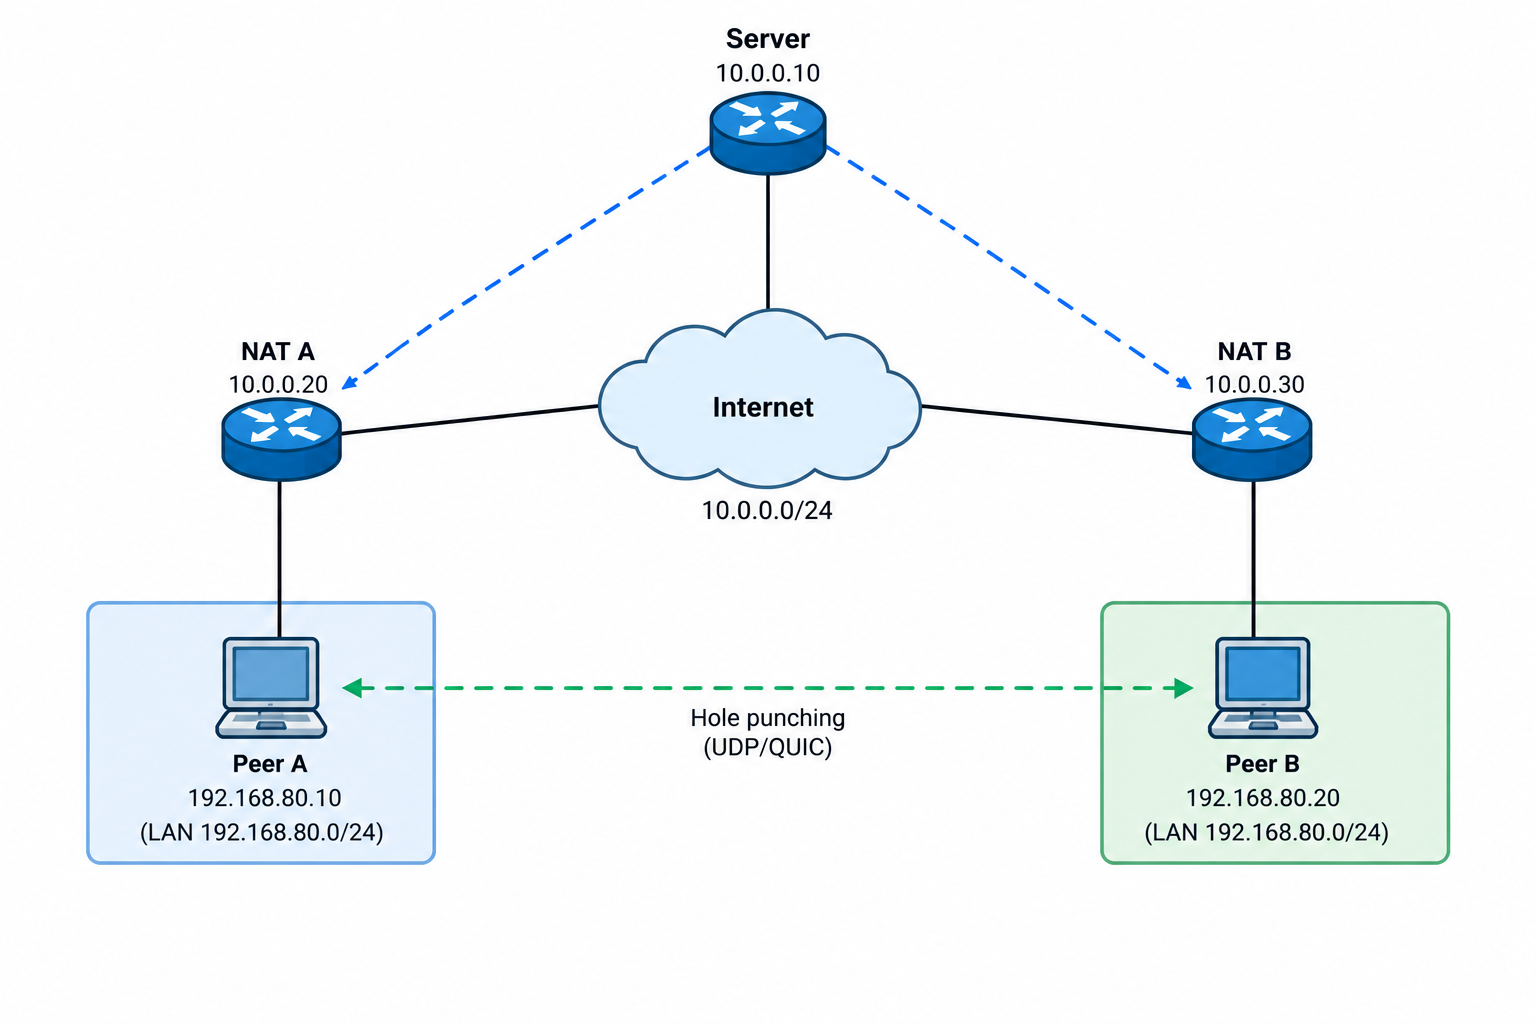
\includegraphics[width=0.8\textwidth]{fig/implementation/topologies/basic_topology.png}
    \caption{Topologia simples para realização de \textit{hole punching}.}
    \label{fig:basic_topology}
\end{figure}

\subsection{Topologia para Hole Punching Utilizando o Protocolo ICE}
\label{sec:ice_topology}

Nesta topologia, os roteadores possuem as mesmas responsabilidades e configurações de NATs  como esperado pelo próprio intuito de uso do ICE de forma a reaproveitar dispositivos já existentes sem que haja a necessidade de alteração destes. Entretanto, os \textit{peers} e o servidor (Server da Figura \ref{fig:basic_topology} obterão novas responsabilidades associas ao processo de estabelecimento de candidatos ICE.

Os \textit{peers} serão incumbidos da responsabilidades associadas a obtenção de candidatos ICE, Essa obtenção, como visto anteriormente na Seção \ref{sec:ice} é possível a partir do protocolo STUN, do protocolo TURN, IPs das interfaces locais, e também IPs descobertos durante a fase dos \textit{connectivity checks}. O \citep{rfc8838} também descreve que estes candidatos não estão limitados a esse escopo e também podem ser obtidos por outros meios. A partir desta obtenção de candidatos, os \textit{peers} também terão a responsabilidade de trocar os IPs candidatos entre si a partir de um servidor de sinalização, que, como descrito anteriormente na Seção \ref{sec:ice}, não faz parte da espectativa do próprio protocolo, portanto uma solução genérica pode ser utilizada (servidor MQTT, servidor HTTP/WebSockets, etc...). E como responsabilidade final, estes \textit{peers} também precisarão realizar os \textit{connectivity checks} do ICE afim de encontrar um possível candidato para a comunicação.

O servidor, nesta topologia, obterá as responsabilidades faltantes para a conclusão do protocolo ICE, portanto este servidor será responsável pela gerência de um servidor STUN, um servidor TURN, e também um servidor de sinalização, a fim de prover os serviços necessários para realização de testes de funcionalidade sobre a implementação proposta entre os demais protocolos.

A topologia continua a mesma, entretanto as responsabilidades aumentam e são dispostas como vistas na Figura \ref{fig:ice_topology}.

\begin{figure}[ht]
    \centering
    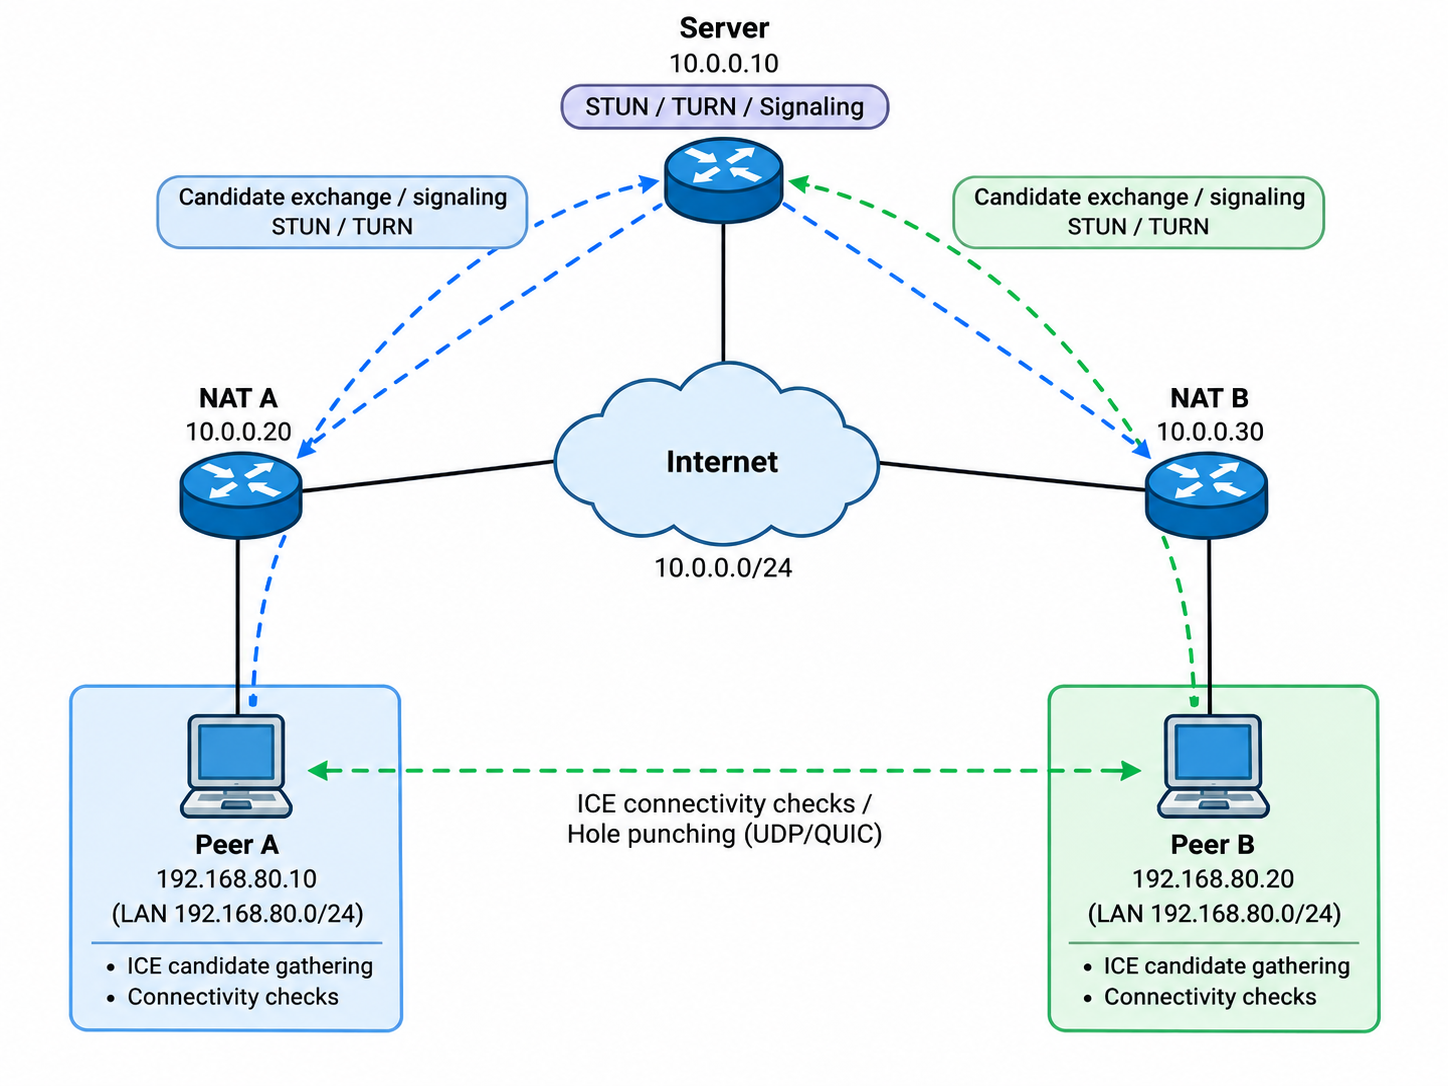
\includegraphics[width=0.8\textwidth]{fig/implementation/topologies/ice_topology.png}
    \caption{Topologia para realização de \textit{hole punching} utilizando o protoclo ICE.}
    \label{fig:ice_topology}
\end{figure}

\section{Ambientes de Simulação}
\label{sec:simulation_environments}

Para a validação das técnicas de \textit{hole punching} utilizando os protocolos propostos na Seção~\ref{sec:hole_punching_protocols}, diferentes ambientes de simulação de rede foram avaliados antes da definição da topologia final de testes (vista na Seção~\ref{sec:topologies}).


\subsection{Ambiente de Simulação GNS3}

O GNS3, ou \textit{Graphical Network Simulator-3}, disponível em \citep{gns3}, é um simulador amplamente utilizado para simulação de redes, permitindo a emulação de dispositivos de rede virtualizados em topologias complexas.

Este simulador foi o primeiro a ser utilizado, devido à familiaridade e ao uso prévio dele em projetos anteriores voltados à universidade. Além disso, a interface gráfica e a integração com o \textit{Wireshark} (ferramenta utilizada para \textit{sniffing} de rede) providas por ele facilitam a análise visual dos pacotes transmitidos, auxiliando na verificação do correto funcionamento das transmissões.

Entretanto, esta ferramenta deixou de ser utilizada à medida que os testes dos protocolos se tornaram mais intensos, devido à sua limitação de integração com o \textit{build system} CMake (ferramenta geradora de sistemas de \textit{build}) desenvolvido para este trabalho, dificultando a automação de testes de regressão.

\subsubsection{Máquinas Virtuais Utilizadas no GNS3}

Para os testes utilizando o GNS3, foram utilizadas máquinas virtuais para simular cada \textit{peer}, NAT e servidor das topologias propostas. Os componentes virtualizados utilizados foram os seguintes:

\begin{itemize}
    \item \textbf{Debian 12.6:} Máquina Debian utilizada para roteadores genéricos e \textit{hosts}, a fim de facilitar a execução de \textit{scripts} e a instalação de bibliotecas;
    \item \textbf{Cisco IOSv 15.9:} Máquina Cisco utilizada como roteador para a simulação e configuração de NATs;
    \item \textbf{NAT:} Componente nativo do GNS3 que simula um NAT de rede. Este componente não é utilizado como NAT alvo do \textit{hole punching}, mas sim para distribuir acesso à internet aos dispositivos internos da topologia, dado que alguns deles necessitam de internet para a instalação de bibliotecas.
\end{itemize}

\subsubsection{Configuração da Topologia Simples para Hole Punching no GNS3}
\label{sec:basic_topology_gns3}

A topologia configurada pode ser vista na Figura~\ref{fig:basic_topology_gns3}. Ela utiliza dois roteadores com NAT de ``mapeamento espelhado'' de porta origem, dois clientes e um servidor (utilizado apenas como \textit{stub} neste momento). Este ``mapeamento espelhado'' se refere ao mapeamento citado na Seção~\ref{sec:basic_topology_hole_punching}, no qual a porta pública é traduzida para a porta de origem. Isso permite que as portas traduzidas sejam conhecidas previamente; do contrário, não seria possível realizar \textit{hole punching} sem a existência de um servidor como o servidor STUN.

\begin{figure}[ht]
    \centering
    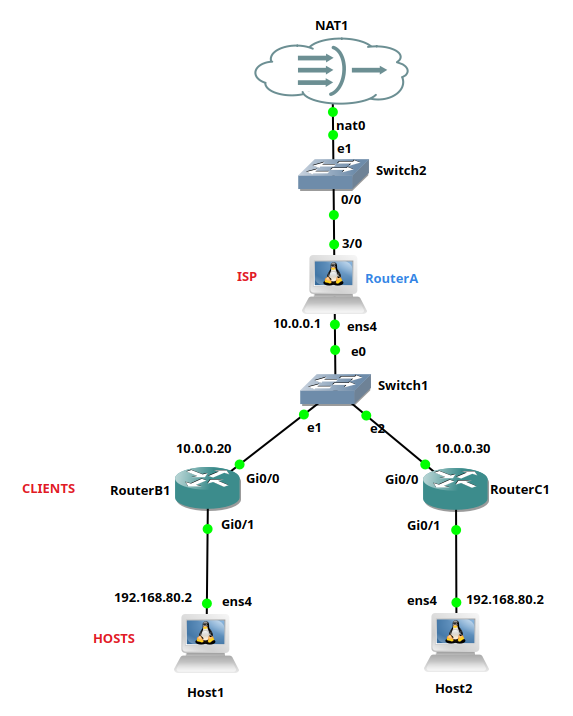
\includegraphics[width=0.6\textwidth]{fig/implementation/gns3/basic_topology_gns3.png}
    \caption{Topologia simples desenvolvida no GNS3.}
    \label{fig:basic_topology_gns3}
\end{figure}

Nesta topologia, todos os \textit{hosts} utilizam o sistema operacional Debian, e cada um deles atua como um \textit{peer} do cenário de \textit{hole punching}. Os NATs são roteadores Cisco IOSv, cada um configurado com um IP público fixo e com mapeamento de portas espelhado em relação à porta dos pacotes de saída, como descrito anteriormente. O ISP é um roteador que, nesta topologia, atua apenas como \textit{stub}, sem participar do \textit{hole punching}, servindo somente como servidor DHCP para os roteadores NAT em uma rede \texttt{10.0.0.0/24}. Já o componente \texttt{NAT1} serve apenas para prover acesso à internet a todos os \textit{peers} abaixo dele.

\begin{comment}
    
\subsubsection{Configuração da Topologia ICE para Hole Punching no GNS3}

Escrever quanto tiver a implementação

\cgk{Implementar a configuração, mas acho que não vale a pena perder tempo}

\end{comment}

\subsection{Linux Network Namespaces}
\label{sec:linux_network_namespaces}

Os \textit{Linux Network Namespaces} (vistos em \citep{linux-network-namespaces}) permitem configurar ambientes de teste na máquina local, utilizando apenas interfaces virtualizadas na comunicação. Os \textit{namespaces} compartilham o mesmo \textit{kernel}, mas possuem isolamento dos recursos de rede, como pode ser visto na Figura~\ref{fig:namespaces_isolation}. Isso facilita a execução de testes de \textit{debug} e de regressão, permitindo a análise de alterações no código que afetam mais do que uma única biblioteca. Este mecanismo foi adotado como principal ambiente de testes devido à sua praticidade.

\begin{figure}[ht]
    \centering
    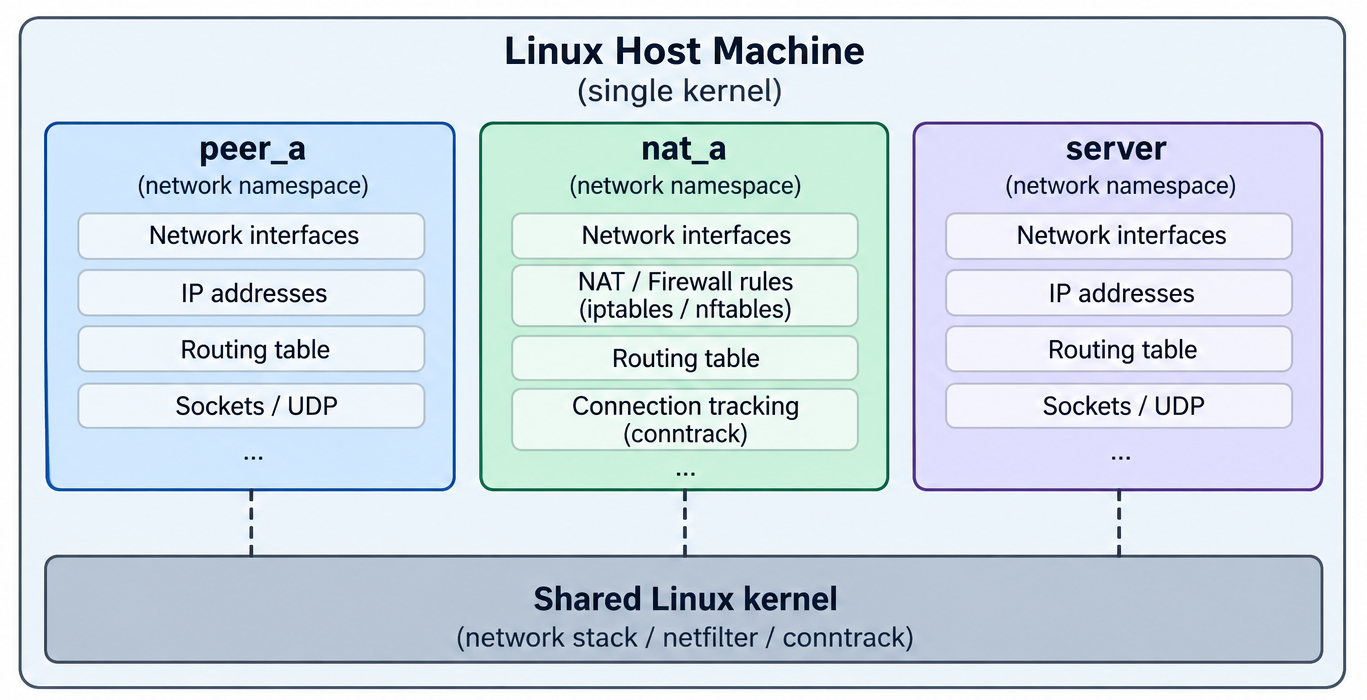
\includegraphics[width=0.8\textwidth]{fig/implementation/network_namespaces/namespaces_isolation.png}
    \caption{Isolamento dos \textit{Network Namespaces} no \textit{kernel} do Linux.}
    \label{fig:namespaces_isolation}
\end{figure}

Entretanto, a configuração nativa desses \textit{namespaces} é feita com o comando \texttt{ip}, que não é trivial de utilizar dado o grande conjunto de configurações possíveis. Por exemplo, para configurar um NAT, além de configurar as interfaces virtuais, é necessário um outro tipo de configuração, feita com o programa \texttt{iptables}. Além disso, a documentação é extensa e não existem perfis pré-configurados para tipos específicos de NAT, como o NAT com EIM ou o NAT com ``mapeamento espelhado''. Por isso, foi escolhido utilizar a biblioteca PatchBay \citep{patchbay}, desenvolvida em Rust, que permite a configuração completa do ambiente a partir de perfis de configuração previamente definidos. Isso facilita os testes e garante o comportamento esperado de cada configuração. Portanto, este trabalho utiliza este \textit{framework} como base das configurações de rede dos \textit{Linux Network Namespaces}.

Nesse ambiente, os nós representam os extremos da comunicação entre \textit{gateways}, sem reproduzir o hardware de dispositivos IoT. Como os \textit{namespaces} compartilham recursos da mesma máquina, os resultados devem ser interpretados de acordo com essa configuração. Os testes nesse ambiente permitem controlar as condições de rede e verificar o funcionamento da integração, enquanto eventual avaliação em hosts separados constitui outro ambiente experimental.

\subsubsection{Topologia Simples para Hole Punching Utilizando Linux Network Namespaces}
\label{sec:basic_topology_network_namespaces}

A topologia simples utilizando \textit{Linux Network Namespaces} é muito parecida com a vista na Figura~\ref{fig:basic_topology_gns3}. A diferença é que o PatchBay não permite a definição manual do IP de WAN dos roteadores NAT; em vez disso, cada roteador recebe um endereço fornecido pelo ISP (como visto na Listagem \ref{lst:patchbay_isp_config}, que neste caso pertence à mesma rede \texttt{10.0.0.0/24}. Cada roteador também atribui endereços IP à sua rede local (LAN) e configura um NAT do tipo \textit{Moderate}.

\begin{lstlisting}[caption={Configuração do ISP no PatchBay.}, label={lst:patchbay_isp_config}]
    let isp = lab
        .add_router("isp")
        .preset(RouterPreset::Public)
        .downstream_cidr("10.0.0.0/24".parse()?)
        .build()
        .await?;
\end{lstlisting}

O PatchBay \citep{patchbay} fornece quatro tipos de NAT para IPv4, além de um modo customizável (\textit{Custom}), de variações para IPv6 e de \textit{firewalls}:

\begin{itemize}
    \item \textbf{None:} Sem NAT, ou seja, um roteador sem qualquer tradução de endereços;
    \item \textbf{Open:} Implementa EIM e EIF, descritos na Seção~\ref{sec:nat_classification_by_translation_behavior}, correspondendo ao \textit{Full-Cone NAT};
    \item \textbf{Moderate:} Implementa EIM e APDF, correspondendo ao \textit{Port-Restricted Cone NAT}. Este é o comportamento típico de roteadores domésticos;
    \item \textbf{Strict:} Implementa EDM (\textit{Endpoint-Dependent Mapping}, com portas aleatórias) e APDF, correspondendo ao \textit{Symmetric NAT}. Quando ambos os \textit{peers} estão atrás desse tipo de NAT, o \textit{hole punching} direto não é possível, sendo necessário um \textit{relay}.
\end{itemize}

Portanto, a topologia implementada utiliza, nos roteadores (clients), o modo \textit{Moderate} como visto na Listagem \ref{lst:patchbay_client_config}, com a alteração de algumas regras de mapeamento para manter o ``mapeamento espelhado'', de modo que a porta traduzida seja, por padrão, a porta de origem do \textit{socket} (definida via \textit{bind}). Desta forma, os \textit{peers} podem permanecer em uma mesma rede local, que neste caso é a mesma vista na Figura~\ref{fig:basic_topology_gns3}, \texttt{192.168.80.0/24}.

\begin{lstlisting}[caption={Configuração de roteadores no PatchBay.}, label={lst:patchbay_client_config}]
    let router_a = lab
        .add_router("router_a")
        .preset(RouterPreset::Home)
        .upstream(isp.id())
        .downstream_cidr("192.168.80.0/24".parse()?)
        .nat(Nat::Moderate)
        .firewall(Firewall::None)
        .build()
        .await?;
\end{lstlisting}

\subsubsection{Configuração da Topologia ICE para Hole Punching utilizando Linux Network Namespaces}
\label{sec:ice_topology_network_namespaces}

A topologia para ICE mantém a disposição dos nós, o endereçamento das redes e o perfil NAT \textit{Moderate} utilizados na topologia básica, descrita na Seção~\ref{sec:basic_topology_network_namespaces}. As regras adicionais de tradução de portas, entretanto, dependem do cenário: os testes sem ICE preservam a porta de origem para permitir o conhecimento prévio dos endpoints públicos; os testes com ICE utilizam a descoberta desses endpoints, incluindo um caso com remapeamento explícito de portas, apresentado na Seção~\ref{sec:experimental_scenarios}. Entretanto, como visto na Seção~\ref{sec:ice_topology}, tanto o servidor quanto os \textit{peers} assumem novas responsabilidades. Na configuração da topologia em si, a configuração dos \textit{peers} não muda, dado que a biblioteca ICE estará integrada ao mesmo \textit{script} já executado anteriormente em cada \textit{peer}. O servidor, entretanto, passará a executar \textit{scripts} que vão além de sua funcionalidade anterior de apenas fornecer o serviço de DHCP.

O servidor passa a assumir duas novas responsabilidades. A primeira está associada ao fornecimento de serviços STUN e TURN, permitindo a cada \textit{peer} a obtenção de mais candidatos públicos a partir desses protocolos. Já a segunda está associada ao fornecimento de um serviço de sinalização, de forma que os \textit{peers} possam trocar candidatos entre si a fim de realizar suas verificações de conectividade.

Para o fornecimento dos serviços STUN e TURN, foi utilizada a biblioteca \texttt{coturn} \citep{coturn}, responsável por implementar serviços coerentes com os RFCs \citep{rfc8489} e \citep{rfc8656}, que trazem as informações mais atualizadas sobre os protocolos e obsoletam comportamentos antigos, tornando-se, portanto, uma solução adequada para a validação da implementação em questão.

Para o fornecimento do serviço de sinalização, o servidor será responsável por executar um \textit{script} simples que realiza a troca de informações entre os \textit{peers}. Este \textit{script} executa um servidor TCP que ouve em todas as interfaces na porta 5555 e aguarda a conexão dos dois \textit{peers}. Assim que os \textit{peers} se conectam, é iniciada a troca de informações entre eles, contendo os dados sobre os candidatos locais de cada \textit{peer}, obtidos por meio do servidor STUN/TURN ou de outro método, juntamente com as informações necessárias para a autenticação prevista no protocolo ICE.

\subsection{Infraestrutura controlada}

Configurar nos roteadores da Datacom...

\cgk{lembrar de adicionar se fizer configurações}

\section{Protocolos de Comunicação para Hole Punching}
\label{sec:hole_punching_protocols}

Este trabalho teve origem em um projeto realizado em conjunto com a Datacom, cujo objetivo era viabilizar a comunicação entre dois \textit{peers} com o mínimo de infraestrutura possível. % Opcional: Com o encerramento do projeto, o trabalho passou a ser continuado em caráter acadêmico, no contexto deste TCC.

Inicialmente, o objetivo era transmitir dados TCP, especificamente HTTP, por meio de técnicas de \textit{hole punching}. Dada a complexidade do TCP \textit{hole punching}, vista na Seção~\ref{sec:tcp_hole_punching}, optou-se pelo UDP \textit{hole punching}. Como base, foi utilizado o Chownat, que, além de realizar \textit{hole punching}, é capaz de tunelar dados TCP sobre UDP sem o custo dos pacotes de controle do TCP, permitindo uma comunicação direta e rápida entre os \textit{peers}.

Para a comunicação, foi proposto o uso de um servidor mínimo (\textit{rendezvous server}), responsável pela autenticação e pela troca de endereços IP entre os \textit{peers}, com função semelhante à de um servidor STUN no que diz respeito à descoberta de endereços. Também foi proposto o uso de um protocolo capaz de garantir os requisitos de dependabilidade e segurança descritos na introdução deste trabalho, tendo-se optado pelo QUIC, dada a sua recente expansão e a compatibilidade com os requisitos de transmissão de dados de aplicação do projeto.

A implementação da infraestrutura de servidores foi realizada apenas parcialmente durante o projeto, e pouco foi desenvolvido da comunicação entre dois \textit{peers} utilizando o QUIC. Este trabalho é também uma extensão do trabalho de Ivan [CITAR TCC DO IVAN], que abordou aspectos mais voltados à segurança e aos objetivos por trás da escolha do QUIC como protocolo ideal para os cenários propostos.

\cgk{Citar o TCC do Ivan}

\begin{comment}
    
No contexto de dispositivos IoT, que podem gerar grandes volumes de dados, a comunicação P2P é um cenário relevante, como descrito na introdução, principalmente em relação ao uso de banda e à necessidade de um servidor especializado para gerenciar o tráfego, além dos requisitos de dependabilidade e segurança para os usuários.

\cgk{Ver se realmente tem trabalhos de IoT relacionados com QUIC e citar aqui}
\end{comment}

No cenário IoT adotado neste trabalho, a comunicação externa é realizada pelos gateways, que executam as aplicações integradas ao túnel. O interesse está em interligar essas aplicações quando os gateways se encontram em redes distintas, utilizando os mecanismos de descoberta e seleção de caminhos disponíveis na solução. Os dados dos dispositivos são representados, nos experimentos, por mensagens geradas por aplicações locais.

Nesta seção são apresentadas as implementações e extensões desenvolvidas para viabilizar a comunicação com as técnicas de \textit{hole punching} propostas inicialmente, possibilitando uma comunicação direta entre dois \textit{peers} atrás de um NAT. 

\begin{itemize}
    \item A Seção \ref{sec:chownat_translation_extension} apresenta uma continuação da implementação desenvolvida durante o projeto;
    \item A Seção \ref{sec:ossl_quic_for_hole_punching} apresenta uma proposta de uso da biblioteca OpenSSL no modo \textit{threadless} para \textit{hole punching}; 
\end{itemize}

\subsection{Interface de transporte para hole punching}
\label{sec:hole_punching_interface}

A interface de transporte para \textit{hole punching} é uma interface criada especificamente para este trabalho, com o intuito de auxiliar a aplicação de múltiplos protocolos de transporte UDP na realização de \textit{hole punching}, independentemente de o protocolo possuir ou não esse recurso de forma nativa. Além disso, esta interface também tem como objetivo habilitar o tunelamento de TCP sobre protocolos de transporte UDP, de modo a transportar pacotes de serviços da camada de aplicação que utilizam TCP sobre protocolos de transporte diferentes.

Esta interface é baseada no Chownat (Seção~\ref{sec:chownat}) e propõe uma abordagem modular desse mesmo protocolo, a fim de permitir reutilizar sua estrutura na aplicação de \textit{hole punching} para outros protocolos, como o QUIC. Como objetivo principal, busca-se permitir o reuso dos componentes do protocolo original (as partes associadas à realização de \textit{hole punching} e ao tunelamento TCP), de forma a permitir apenas ``trocar peças'' e facilitar a integração de outros protocolos.

Esta interface também propõe uma abordagem \textit{threadless}, a partir de uma API baseada em eventos, similar à provida pela \texttt{libwebsockets} \citep{libwebsockets},
que serviu como inspiração para a API desenvolvida. Esta implementação baseada em eventos utiliza chamadas de sistema por meio da \textit{syscall} \texttt{select}, que permite a integração de múltiplos \textit{sockets} e a espera por novos dados recebidos neles.

Além disso, esta interface também permite um modelo de configuração que possibilita a gerência tanto da configuração quanto do uso de \textit{hole punching}, bem como do uso de tunelamento TCP. Isto é feito de forma prévia ao início real da conexão do protocolo, o que também favorece a arquitetura modular.

\subsubsection{Configuração da interface}

A configuração da interface permite, assim como o próprio Chownat visto anteriormente, a existência de duas sessões: uma sessão UDP e uma sessão TCP, possibilitando o tunelamento.

Cada sessão possui configurações específicas para a devida conexão, como \textit{timeouts} e endereços de origem e destino. Isto permite que uma aplicação que utilize esta interface possa configurá-la previamente a partir de dados obtidos de forma externa, como, por exemplo, a partir do ICE.

A configuração também permite o registro de uma \textit{callback}, que será chamada a cada novo evento, passando como parâmetro o \textit{reason} (motivo) do evento específico.

Para fornecer uma organização baseada no paradigma de orientação a objetos, a configuração também permite que seja escolhida uma implementação específica de protocolo que utilizará a sessão UDP. Isso significa que um novo protocolo UDP que deseje utilizar esta mesma interface precisa apenas implementar um conjunto de funções pré-definidas, simulando o comportamento de uma tabela virtual. Na prática, essa tabela é representada por um conjunto de ponteiros de função, que devem ser implementados por cada implementação de protocolo UDP com interesse em utilizar a interface. A API pública da interface pode ser observada diagrama de blocos visto na Figura \ref{fig:udp_conn_diagram}.

\begin{figure}[ht]
    \centering
    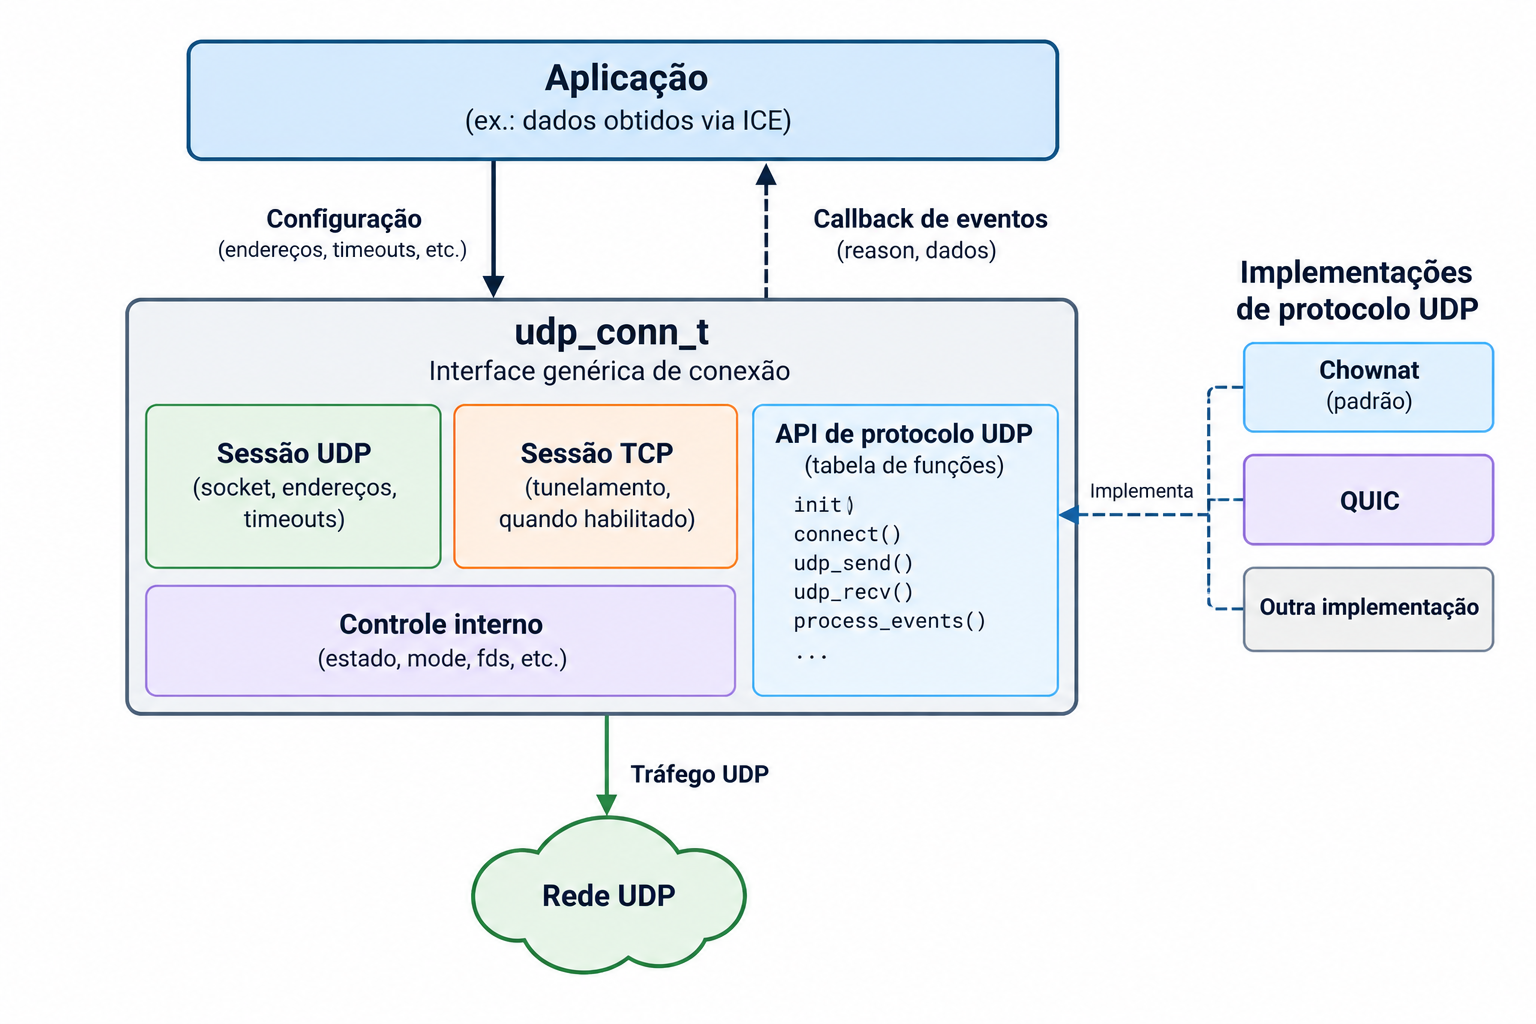
\includegraphics[width=0.8\textwidth]{fig/implementation/interface/udp_conn_diagram.png}
    \caption{Diagrama de blocos da interface genérica de conexão UDP udp\_conn\_t.}
    \label{fig:udp_conn_diagram}
\end{figure}

Além disso, esta interface genérica permite que o protocolo UDP que roda sobre ela funcione em dois modos: o modo cliente e o modo servidor. Cada um dos modos possui determinadas funções quando se está fazendo uso do tunelamento TCP. Esses mesmos comportamentos são os vistos na Seção~\ref{sec:chownat} e também serão abordados na próxima seção.

\subsubsection{Fluxo de conexão e hole punching}
\label{sec:interface_connection_flow_and_hole_punching}

A conexão utilizando esta interface se baseia em três operações diferentes; a ordem dessas operações é o que define se o processo está operando como cliente ou servidor. Portanto, dependendo do modo de operação da interface, essas operações são chamadas em uma ordem diferente. As operações utilizadas nesse processo são:

\begin{enumerate}
    \item \textbf{Bind TCP:} Responsável pelo vínculo da sessão TCP com o serviço local;
    \item \textbf{Hole Punching:} Realização de NAT traversal por UDP hole punching;
    \item \textbf{Conexão UDP:} Processo de conexão do protocolo em si, caso não integrado com \textit{hole punching}.
\end{enumerate}

Para entender essas diferenças, é importante retomar as etapas de conexão já descritas na Seção~\ref{sec:chownat_connection}. No modo cliente, aguarda-se uma conexão TCP realizada por um outro processo na própria máquina para o serviço desejado, enquanto, no modo servidor, apenas se espera por uma conexão UDP remota. Da mesma forma, após o recebimento da conexão UDP, o cliente inicia o \textit{hole punching}; já o servidor, após completar o \textit{hole punching}, conecta-se ao serviço TCP local. Isto implica uma ordem invertida entre essas duas operações, gerando o fluxo que pode ser visto na Figura~\ref{fig:udp_conn_connection_flow_diagram}:

\begin{figure}[ht]
    \centering
    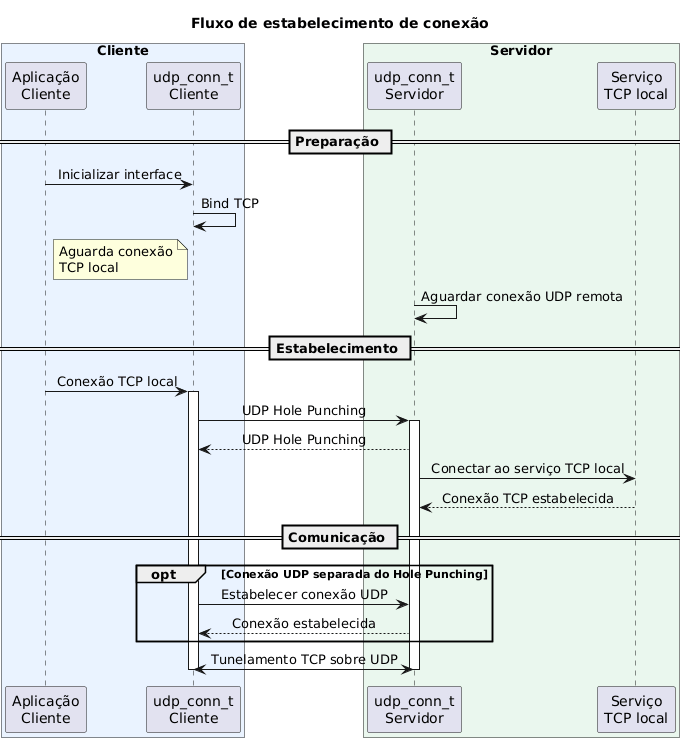
\includegraphics[width=0.8\textwidth]{fig/implementation/interface/udp_conn_connection_flow_diagram.png}
    \caption{Diagrama de tempo da interface de conexão UDP \texttt{udp\_conn\_t}.}
    \label{fig:udp_conn_connection_flow_diagram}
\end{figure}

Importante destacar que a implementação do protocolo UDP é responsável apenas pelas etapas que envolvem a comunicação externa com o outro \textit{peer}. Ou seja, as comunicações TCP internas ficam gerenciadas diretamente pela própria interface, abstraindo do protocolo a necessidade de conhecimento sobre o funcionamento do tunelamento.

\subsubsection{API e loop de eventos}
\label{sec:api_and_event_loop}

A API baseada em eventos é uma adição ao protocolo Chownat, permitindo um comportamento reativo, além de possibilitar o uso do protocolo sem que haja tunelamento TCP. Isso faz parte da extensão do protocolo Chownat implementada, descrita mais detalhadamente na Seção~\ref{sec:chownat_translation_extension}.

Existem dois níveis de recebimento de eventos. O primeiro são os eventos indicados pelo sistema operacional à própria interface, para indicar que um novo pacote foi recebido em uma determinada \textit{socket}. Isto é feito por meio da chamada de sistema \textit{select}, que permite a espera em um subconjunto de \textit{sockets}, gerando um evento para a interface e permitindo que ela continue executando a partir dessa chamada. Esta chamada já era utilizada no Chownat, e é um dos principais mecanismos que permite o \textit{hole punching} a partir do envio de pacotes \textit{keep-alive}, como visto na Listagem~\ref{lst:select_pseudocode}.

\begin{lstlisting}[caption={Pseudocódigo do loop de eventos da interface}, label={lst:select_pseudocode}]
    while (true)
        ret = select(sockets, ..., timeout)
        if (ret == TIMEOUT_EXCEEDED)
            send_keep_alive()
        else
            handle_sockets()
\end{lstlisting}

O outro nível são os eventos recebidos pela própria aplicação. Estes eventos são determinados por cada implementação de protocolo, dado que cada uma pode possuir diferentes tipos de eventos, podendo ser o recebimento de determinada mensagem, de determinado erro, início e fim de conexão, etc. Isso permite que a aplicação possa interferir no fluxo de conexão em determinados momentos, a partir da API pública da interface, que inclui as seguintes ações:

\begin{itemize}
    \item \textbf{udp\_conn\_send:} Enviar mensagem;
    \item \textbf{udp\_conn\_recv:} Esperar recebimento de mensagem;
    \item \textbf{udp\_conn\_disconnect:} Finalizar conexão.
\end{itemize}

Além desta API pública, existem ainda as funções de criação de conexão, que não são permitidas dentro do \textit{loop} de eventos, sendo elas:

\begin{itemize}
    \item \textbf{udp\_conn\_init:} Inicializa a interface com determinada implementação;
    \item \textbf{udp\_connection:} Inicializa a conexão. É o próprio \textit{loop} de eventos; ao entrar nessa função, só sai dela se a conexão for finalizada;
    \item \textbf{udp\_conn\_deinit:} Desinicializa a interface.
\end{itemize}

\subsubsection{Tunelamento TCP}

O tunelamento TCP é um dos principais atributos da arquitetura do Chownat, permitindo a conectividade entre \textit{peers} e o reuso de serviços já implementados sobre TCP, com menor \textit{overhead} de comunicação, modularidade dos serviços (pois desacopla, de forma indireta, o protocolo de transporte) e facilidade de migração de serviços baseados em TCP para UDP. Essa facilidade de migração representa uma característica relevante para a proposta deste trabalho, considerando a ampla utilização de protocolos de aplicação baseados em TCP e em arquiteturas cliente-servidor no contexto da Internet das Coisas (IoT), como HTTP e MQTT. Dessa forma, a solução proposta busca facilitar a adoção de uma arquitetura \textit{peer-to-peer} por aplicações existentes, reduzindo a necessidade de modificações nos serviços originalmente desenvolvidos para comunicação sobre TCP.

A interface permite o uso de técnicas de tunelamento de forma transparente à implementação do protocolo, mantendo-o como um atributo opcional para a aplicação que fará uso da interface. Como visto anteriormente na Seção~\ref{sec:chownat}, a conexão TCP ocorre apenas de forma local, e os pacotes produzidos pelo serviço são enviados à interface por meio de uma \textit{socket} TCP vinculada ao serviço em execução, permitindo que segmentos de controle TCP (como ACKs, FIN, SYN) existam apenas localmente, mantendo, para a conexão remota externa, apenas o envio de dados do serviço de aplicação (HTTP, SSH, etc.). Entretanto o protocolo UDP pode transmitir seus próprios pacotes de controle. Quando a aplicação envia uma mensagem para a \textit{socket} vinculada, o \textit{loop} de eventos da interface (visto na Seção~\ref{sec:api_and_event_loop}) é ativado, avisando-a do recebimento da mensagem em uma das \textit{sockets}. É então analisado em qual \textit{socket} o pacote foi recebido: caso seja na \textit{socket} TCP, os dados do pacote são coletados e enviados através da implementação UDP. Ao receber um pacote do \textit{loop} de eventos da interface, caso ele seja UDP, basta retornar os dados à interface, que será responsável por verificar a existência de tunelamento e redirecionar os dados recebidos para a \textit{socket} TCP local, permitindo uma resposta à aplicação. Este fluxo completo pode ser visto na Figura~\ref{fig:udp_conn_tcp_tunneling_diagram}.

\begin{figure}[ht]
    \centering
    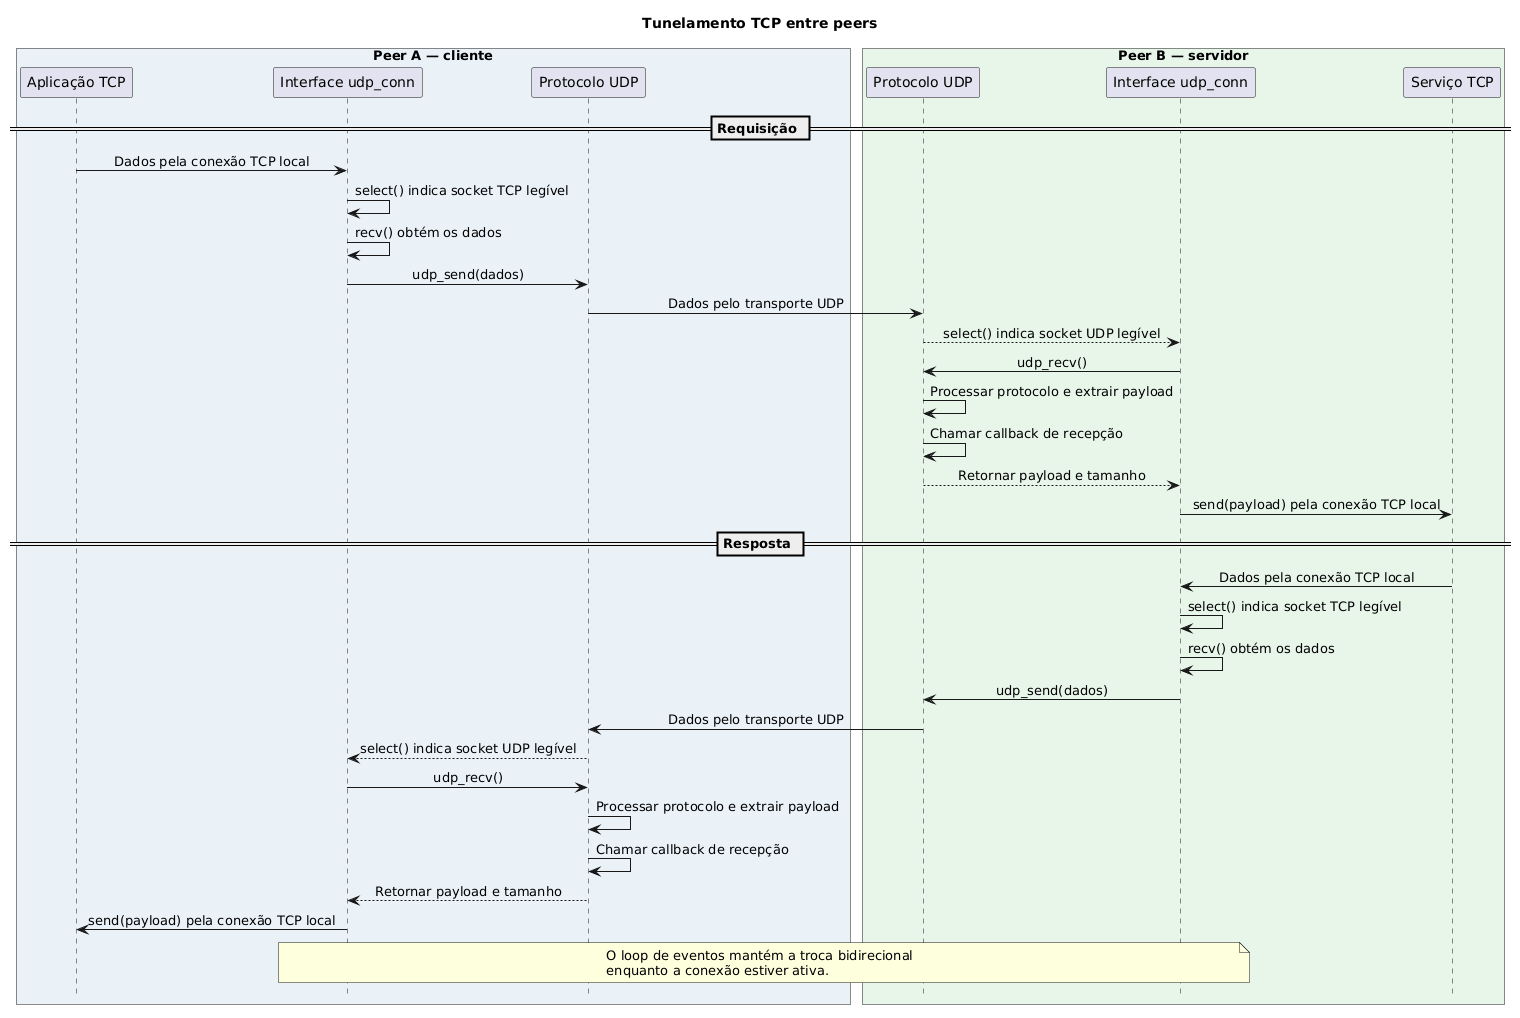
\includegraphics[width=1.0\textwidth]{fig/implementation/interface/udp_conn_tcp_tunneling_diagram.png}
    \caption{Diagrama de tempo de uma requisição TCP tunelada por UDP utilizando a interface udp\_conn\_t.}
    \label{fig:udp_conn_tcp_tunneling_diagram}
\end{figure}

No cenário considerado, a aplicação integrada ao túnel executa no próprio gateway. Ela utiliza uma conexão TCP local para entregar e receber os dados transportados entre os hosts. A obtenção desses dados a partir de sensores, assim como seu encaminhamento a atuadores locais, pertence à aplicação do gateway e não é implementada pelo túnel. Nos experimentos, essas funções são abstraídas por aplicações locais de geração e recepção de mensagens.

\subsection{Tradução e Extensão do Protocolo Chownat}
\label{sec:chownat_translation_extension}

O protocolo Chownat, como visto anteriormente, é nativo em Perl, disponível em \citep{kamkar2004chownatv07}. Durante o projeto da Datacom descrito no início desta seção, foi escolhido o uso deste protocolo, dado que ele era capaz de suprir as necessidades momentâneas para compreensão e aplicação de técnicas de NAT traversal, assim como pela existência do \textit{hole punching} de forma nativa ao protocolo, além do tunelamento TCP, que permitia o tráfego TCP necessário para as aplicações HTTP do projeto.

Durante o projeto com a Datacom, foi feita uma tradução do protocolo para C e Dart, de forma a manter sua forma nativa de funcionamento, sem extensões e sem modificações, apenas replicação da funcionalidade. Entretanto, a tradução não havia sido feita de forma completa, e possuía diversas limitações, principalmente associadas às etapas de criação, reinício e finalização de conexões. Além disso, por conta do propósito inicial do Chownat possuir apenas tunelamento TCP, não era possível utilizar uma comunicação apenas com UDP.

O objetivo do desenvolvimento de extensões e modificações no próprio Chownat, apesar de este não ser o objetivo principal do trabalho, foi a realização de testes de funcionamento e a generalização da própria interface (vista na Seção~\ref{sec:hole_punching_interface}) para protocolos posteriores, como o QUIC. Portanto, o valor desse desenvolvimento está associado muito mais à garantia de funcionamento do que à real sugestão de uso deste protocolo para qualquer tipo de aplicação posterior, dadas as diversas limitações, como a falta de garantia dos requisitos de dependabilidade (citados na introdução deste trabalho) cruciais na transmissão de dados da comunicação IoT.

\subsubsection{Limitações do Chownat e extensões desenvolvidas}
\label{sec:chownat_limitations}

O protocolo Chownat possui diversas limitações, principalmente associadas ao seu objetivo original. No momento de seu desenvolvimento (2004) \citep{kamkar2004chownat}, técnicas de NAT traversal ainda estavam sendo exploradas, e o uso de arquiteturas de rede P2P ainda era mal visto, devido ao seu histórico de uso em contextos de pirataria. Portanto, o objetivo principal do Chownat não parece ter sido pensado para o uso contínuo em um dispositivo, mas sim principalmente para provar o funcionamento de técnicas de \textit{hole punching} sobre dispositivos NAT.

Dado que a interface genérica apresentada na Seção~\ref{sec:hole_punching_interface} foi baseada inicialmente no protocolo Chownat, foram propostos alguns mecanismos para generalizar a interface e viabilizar seu uso completo por outros protocolos, o que implica que o próprio Chownat também passa a se beneficiar dessas mudanças. Nem todas as limitações foram solucionadas, principalmente por serem específicas do protocolo, como suas próprias garantias de dependabilidade; ainda assim, parte delas foi resolvida para permitir a realização de testes sobre os recursos da interface. As principais limitações, e o tratamento dado a cada uma, são:

\begin{itemize}
    \item \textbf{Conexão suporta apenas o envio de 256 pacotes:} existe apenas um único byte de representação de identificador de pacote, portanto existem apenas valores possíveis entre 0 e $2^8-1$ para os identificadores. Optou-se por manter o mesmo cabeçalho do Chownat (Seção~\ref{sec:chownat_protocol}), reinicializando a contagem de pacotes ao atingir o limite; perdas de mais de 256 pacotes consecutivos ainda geram comportamento indefinido, mas essa solução foi preferida a estender o campo para 2 bytes, preservando o formato original do pacote;
    \item \textbf{Apenas permite comunicação de dados TCP:} o protocolo Chownat funciona apenas tunelando TCP, não sendo possível o envio nativo de dados UDP sem a existência do tunelamento. Com a criação da interface genérica, o tunelamento TCP passou a ser opcional por conexão, permitindo que a aplicação envie dados nativamente, sem depender de uma conexão TCP externa;
    \item \textbf{Permite apenas uma conexão por aplicação:} ao finalizar a única conexão TCP suportada, o protocolo original entrava em \textit{loop} infinito. Isso foi resolvido com a implementação de um \textit{3-way-handshake} de desconexão, com número máximo de tentativas configurável por conexão, permitindo que, ao finalizar uma conexão TCP, a conexão Chownat também seja finalizada e uma nova conexão possa ser inicializada;
    \item \textbf{Hole punching exige tradução de porta com ``mapeamento espelhado'':} o \textit{hole punching} do Chownat depende de o mapeamento das portas seguir uma regra específica, traduzindo-as exatamente para a porta de origem vinculada pela \textit{socket} que enviará o pacote UDP. Na prática, alguns NATs assumem esse comportamento, como o NAT simulado pelo PatchBay \citep{patchbay} no modo \textit{Moderate}, mas trata-se de um caso particular, e não de uma regra geral entre implementações de NAT. Este problema foi posteriormente resolvido com a integração da biblioteca ICE, descrita na Seção~\ref{sec:ice_library};
    \item \textbf{Sem garantias de dependabilidade:} o protocolo não possui qualquer garantia de confiabilidade, integridade, autenticidade e segurança. Esse problema não foi resolvido, dado que o objetivo final é o uso do protocolo QUIC, que oferece nativamente mecanismos de entrega confiável e proteção criptográficare, mantendo-se, portanto, a simplicidade do Chownat para fins exclusivos de teste.
\end{itemize}

Em síntese, as extensões desenvolvidas não transformam o Chownat em um protocolo pronto para uso em produção, sua limitação mais fundamental, a ausência de garantias de dependabilidade, foi deliberadamente deixada sem solução. O valor desse trabalho de extensão está em ter viabilizado um protocolo funcional e já conhecido como base de testes para a interface genérica proposta neste trabalho, permitindo validar empiricamente as técnicas de \textit{hole punching} antes de aplicá-las a um protocolo com garantias mais robustas, como o QUIC.

\subsection{Uso da Biblioteca OpenSSL para QUIC Hole Punching}
\label{sec:ossl_quic_for_hole_punching}

Dada a complexidade do protocolo QUIC, como visto anteriormente no Capítulo~\ref{chap:quic}, optou-se por utilizar uma biblioteca para realizar a comunicação entre \textit{peers} utilizando este protocolo. Além disso, o protocolo possui diversas características associadas à segurança, o que contribui como outro fator contrário à implementação própria, de forma a evitar riscos de segurança associados a qualquer falha de implementação.

Dado o objetivo de utilizar uma arquitetura baseada no protocolo Chownat, optou-se por não utilizar uma implementação já existente de QUIC hole punching, pois estas seguem abordagens diferentes, como a realização de alterações no próprio protocolo QUIC, a exemplo da segunda proposta de \citep{draft-seemann-quic-nat-traversal}. Portanto, o objetivo foi utilizar uma biblioteca já implementada e bem estabelecida para a realização da primeira alternativa de QUIC \textit{hole punching} proposta por \citep{draft-seemann-quic-nat-traversal}, que se resume em realizar o \textit{hole punching} previamente, via ICE ou outro método equivalente, seguido da transição para a conexão QUIC sobre o caminho já estabelecido.

Para a implementação do protocolo QUIC, optou-se pela utilização da biblioteca OpenSSL, um projeto de código aberto consolidado no desenvolvimento de soluções criptográficas e protocolos de comunicação segura. A partir da versão 3.2, disponibilizada em novembro de 2023 (como visto por \citep{openssl_quic}), a OpenSSL passou a oferecer suporte nativo a conexões QUIC no lado cliente, posteriormente expandido para o lado servidor na versão 3.5. A escolha dessa biblioteca fundamenta-se na manutenção ativa do projeto, na disponibilidade de documentação oficial e na integração do protocolo QUIC à API SSL já existente, permitindo reutilizar abstrações e mecanismos de comunicação disponibilizados pela biblioteca. Além disso, a biblioteca OpenSSL permite o uso de uma \textit{socket} externa, possibilitando reutilizar uma \textit{socket} que, por exemplo, já tenha passado por \textit{hole punching}, mantendo o caminho aberto para a conexão QUIC, o que é um pré-requisito para o uso da abordagem baseada na arquitetura Chownat com a primeira alternativa proposta por \citep{draft-seemann-quic-nat-traversal}, dado que não há alterações na implementação original do protocolo.

A plataforma de execução considerada é o \textit{host} que representa o \textit{gateway}. A escolha das bibliotecas prioriza os recursos necessários à integração e à avaliação do transporte. O trabalho não estabelece requisitos mínimos de execução nem caracteriza o consumo dessas dependências em dispositivos IoT com recursos limitados.

\subsubsection{Configuração e conexão do protocolo QUIC}

Para a configuração, a implementação do protocolo sobre a interface expõe parte da API da OpenSSL; portanto, nem todos os recursos disponibilizados estão acessíveis, e a implementação funciona mais como um \textit{wrapper}, adicionando algumas configurações à API que simplificam o uso para o usuário. Esta implementação \textit{wrapper} foi denominada com o nome ``ossl\_quic''. O usuário poderá configurar, tanto para o cliente quanto para o servidor, as suítes de criptografia disponibilizadas pela OpenSSL para o TLS 1.3, que é o único protocolo de criptografia disponível para a comunicação QUIC.

A implementação da OpenSSL é baseada em contextos, e cada contexto permite uma série de configurações diferentes. As configurações para cliente e servidor diferem, principalmente por não estar sendo utilizada a variante de mTLS (\textit{Mutual Transport Layer Security}), responsável pela garantia de autenticidade tanto do servidor quanto do cliente. Nos experimentos, foi utilizado um certificado autoassinado e a validação do certificado pelo cliente foi desabilitada. Essa configuração permite o estabelecimento da conexão cifrada, mas não verifica a identidade do servidor remoto. Seu uso foi restrito aos testes e é desaconselhado em ambientes de produção. Em ambientes de produção, a validação do certificado deve estar habilitada, com uma configuração de confiança adequada para verificar a identidade do servidor remoto.

Além disso, apesar de não ter sido abordado no Capítulo~\ref{chap:quic}, o QUIC também permite a configuração de um protocolo de aplicação a partir da ALPN (\textit{Application Layer Protocol Negotiation}), a fim de definir um protocolo acordado para uso durante a negociação da conexão. Neste caso, essa configuração não é estritamente necessária, pois o objetivo é apenas o transporte de dados genéricos, não associados a um protocolo específico; para isso, utiliza-se apenas um nome arbitrário, escolhido como sendo ``osslquic''.

Assim como no Chownat, esta etapa inicial inicializa a \textit{socket} UDP, vinculando-a a um endereço específico, da mesma forma descrita na Seção~\ref{sec:chownat}. O diagrama de tempo desta configuração pode ser visto na Figura~\ref{fig:ossl_quic_configuration}.

\begin{figure}[ht]
    \centering
    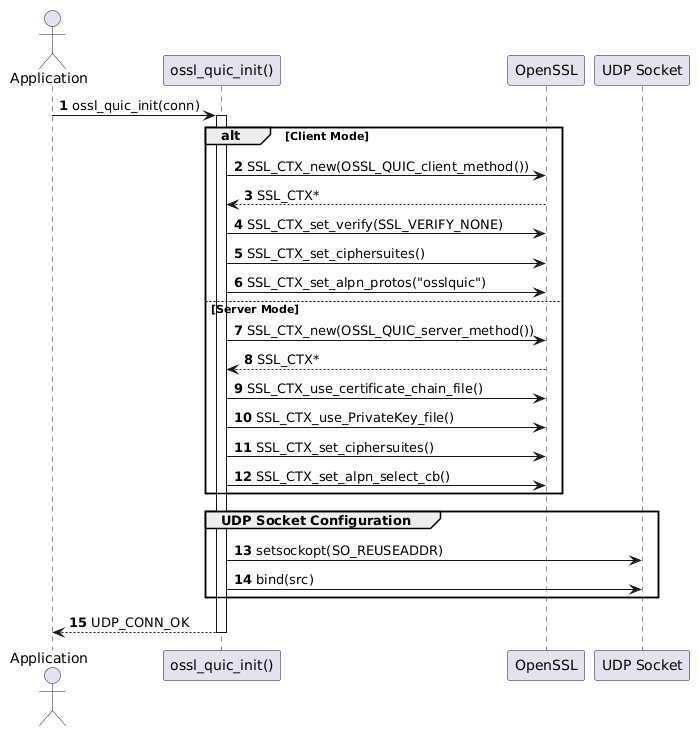
\includegraphics[width=0.8\textwidth]{fig/implementation/ossl_quic/ossl_quic_configuration_time_diagram.png}
    \caption{Diagrama de tempo da configuração do QUIC da OpenSSL sobre a interface.}
    \label{fig:ossl_quic_configuration}
\end{figure}

\subsubsection{Processo de hole punching e conexão}

O processo de \textit{hole punching} da implementação ``ossl\_quic'' segue o mesmo padrão visto no Chownat: o objetivo central é a realização do \textit{hole punching} de forma prévia à conexão QUIC, implementando assim, de forma parcial, a primeira proposta descrita por \citep{draft-seemann-quic-nat-traversal}. Na prática, este \textit{hole punching} pode ser realizado utilizando o próprio ICE, como descrito na Seção~\ref{sec:ice_library}.

Após a realização do \textit{hole punching} por si só, inicia-se a conexão QUIC. Isto implica a implementação da etapa opcional de conexão UDP, descrita na Seção~\ref{sec:interface_connection_flow_and_hole_punching} e ilustrada na Figura~\ref{fig:udp_conn_connection_flow_diagram}. Para a realização desta operação, é primeiro necessário executar uma operação interna da implementação, chamada por este trabalho de \textit{pre connect}. Além disso, é relevante relembrar que não é necessário realizar o descarte de pacotes manualmente, pois, como visto na Seção~\ref{sec:quic_long_header_packets}, que se baseia em \citep{rfc9000}, pacotes \texttt{Initial} recebidos pela \textit{engine} do QUIC que possuam tamanho menor que 1200 bytes já são descartados automaticamente por ela.

A \textit{pre connect} é uma operação realizada antes da conexão, como o próprio nome sugere, sendo responsável por criar uma nova conexão SSL (nome dado às conexões da OpenSSL), posteriormente utilizada para realizar a conexão QUIC. Esta operação executa três ações principais: cria a conexão (ou \textit{listener}, no caso do servidor); inicializa cada um desses objetos em seu devido estado; e vincula o FD (\textit{file descriptor}) correspondente, configurando a conexão do cliente como cliente e a do servidor como \textit{listener}. Além disso, no lado do cliente, é chamada a função \texttt{connect} da POSIX, responsável por vincular uma \textit{socket} UDP a um endereço remoto, sem necessariamente realizar uma conexão (diferentemente do que ocorreria com TCP). Já no lado do servidor, a \textit{socket} é configurada inicialmente como bloqueante, para que o servidor aguarde pela própria conexão QUIC.

Durante a conexão, o QUIC no modo servidor apenas aguarda, com um \texttt{accept}, até receber uma conexão externa, enquanto no modo cliente é iniciada uma operação de conexão utilizando a biblioteca OpenSSL. Esta operação de conexão realiza as etapas descritas na Seção~\ref{sec:quic_connection_steps}.

\subsubsection{Gerência da conexão}

A gerência da conexão ocorre da mesma forma que a vista no Chownat, na Seção~\ref{sec:chownat}, através do uso de \textit{keep-alives} e do envio de mensagens por chamadas \texttt{send} e \texttt{recv}, além da gerência do tunelamento TCP já discutida anteriormente. Entretanto, por conta de a \textit{engine} QUIC provida pela OpenSSL ser mais elaborada do que um protocolo simples como o Chownat, foi necessária uma extensão da interface descrita na Seção~\ref{sec:hole_punching_interface}, de forma a suportar possíveis comportamentos da implementação do protocolo. Esta extensão da interface incluiu o processamento de possíveis eventos, em conjunto com o processamento de possíveis dados pendentes do protocolo.

O processamento de eventos é necessário dado que a interface é \textit{threadless}, como visto anteriormente na Seção~\ref{sec:hole_punching_interface}. Isto implica que eventos assíncronos, como \textit{timeouts} ou o tratamento do recebimento e envio de pacotes de controle, precisam ser processados explicitamente pela própria interface. Como descrito por \citep{openssl_ssl_handle_events}, isso não seria necessário caso a biblioteca estivesse configurada para o modo de assistência por \textit{threads}, já que, nesse modo, a \textit{thread} de controle da biblioteca seria periodicamente responsável pelo tratamento desses eventos. Estes eventos também são gerenciados nas chamadas de \textit{read} e \textit{write}, que operam em modo bloqueante apenas dur103ante a etapa de conexão, sendo não bloqueantes em todos os demais momentos. Importante destacar que, mesmo no modo bloqueante, ainda é necessário o tratamento de eventos quando as chamadas de \textit{read} e \textit{write} ocorrem apenas após longos períodos de tempo.

O processamento de dados pendentes, por sua vez, decorre de um comportamento específico da biblioteca OpenSSL. Ao receber um conjunto de pacotes QUIC, seja através do processamento de eventos, seja a partir de operações de \textit{read}, a biblioteca armazena esses pacotes em um \textit{buffer} interno de sua própria implementação, deixando dados pendentes de leitura que, no entanto, não são mais lidos diretamente da \textit{socket}, e sim da própria biblioteca. Na abordagem original do Chownat, a espera por dados dependia inteiramente da existência de dados na \textit{socket}, verificada pelo \textit{loop} de eventos. Ao utilizar a biblioteca QUIC, entretanto, essa mesma lógica de espera na \textit{socket} passa a ser insuficiente: a \textit{socket} é considerada vazia assim que a OpenSSL a esvazia internamente, mesmo que outros pacotes tenham chegado e sido armazenados no \textit{buffer} interno da biblioteca, ainda pendentes de processamento. Por esse motivo, também se faz necessário o processamento desses dados pendentes na própria implementação interna da interface.

Além disso, ao ser adicionado o processamento de eventos, uma segunda dependência temporal passa a existir na interface. Inicialmente, a única dependência temporal era o \textit{timeout} de atividade nas \textit{sockets}, controlado pela chamada de sistema \textit{select}; com a extensão, passa a existir também o \textit{timeout} para a ocorrência de eventos internos, gerenciado pela própria implementação da OpenSSL. Isto implica que o tempo de espera do \textit{select} pode precisar ser mais curto, em função da necessidade de tratar um evento interno do protocolo antes do próximo \textit{keep-alive}.

A forma como isso foi resolvido consiste em manter um ponto de referência de inatividade, atualizado sempre que ocorre atividade na \textit{socket}. A cada iteração, os dois \textit{timeouts} são comparados, e o menor entre eles é utilizado como tempo de espera do \textit{select}. Ao ocorrer um \textit{timeout} do \textit{select}, verifica-se se o ponto de inatividade já foi atingido ou ultrapassado: em caso afirmativo, o \textit{timeout} ocorreu por inatividade, e um \textit{keep-alive} é enviado para manter o mapeamento do NAT. Caso contrário, o \textit{timeout} foi causado pelo \textit{timeout} interno de eventos, mais curto; nesse caso, o \textit{loop} retorna ao início e processa os eventos e pacotes pendentes antes de aguardar novamente pelo próximo pacote no \textit{select}.

Desta forma, o fluxo visto previamente na Figura~\ref{fig:udp_conn_tcp_tunneling_diagram} recebe algumas alterações, de forma a se manter portável para bibliotecas com certos requisitos não exigidos nem tratados anteriormente pelo Chownat, devido à sua simplicidade. Isto resulta em um fluxo com os passos vistos na Figura~\ref{fig:udp_conn_additional_methods}.

\begin{figure}[!ht]
    \centering
    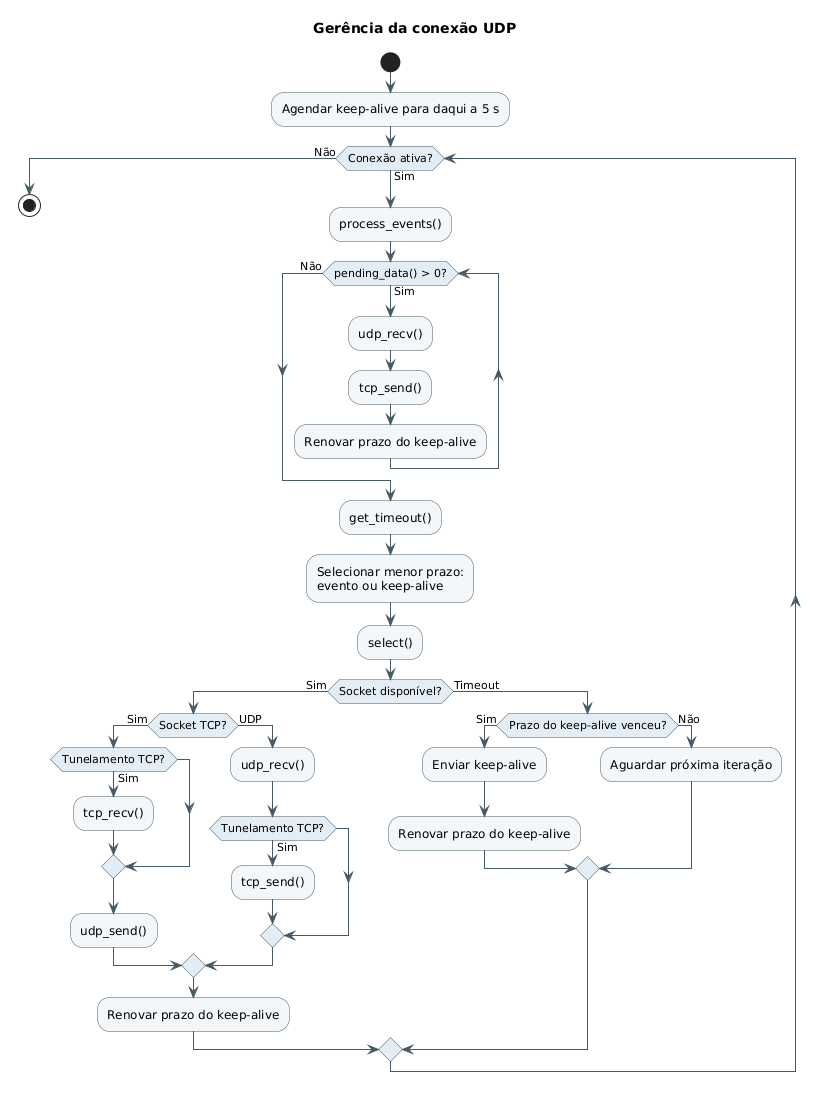
\includegraphics[width=0.8\textwidth]{fig/implementation/ossl_quic/new_udp_conn_diagram.png}
    \caption{Diagrama de atividades do fluxo atualizado da interface \texttt{udp\_conn\_t}.}
    \label{fig:udp_conn_additional_methods}
\end{figure}

\section{Uso da Biblioteca libnice para a Integração do Protocolo ICE}
\label{sec:ice_library}

Como visto anteriormente na Seção~\ref{sec:ice}, o protocolo ICE é o protocolo responsável pela descoberta prévia dos endereços IP de cada \textit{peer} que deseja realizar uma comunicação P2P a partir de técnicas de NAT traversal. A implementação descrita até então na Seção~\ref{sec:hole_punching_protocols} herda do protocolo Chownat a dependência do conhecimento prévio desses endereços pelo \textit{peer}. Isto implica a dependência chamada por este trabalho de ``mapeamento espelhado'', também descrita na Seção~\ref{sec:chownat_limitations}. Como forma de propor uma solução genérica para este problema, tanto para o próprio Chownat quanto para protocolos que herdam a interface genérica \texttt{udp\_conn} descrita na Seção~\ref{sec:hole_punching_interface}, foi criada uma nova interface de transporte, responsável pela gerência da \textit{socket} UDP da conexão, que permite à aplicação escolher o modelo de protocolo de transporte, suportando tanto a abordagem legada descrita na Seção~\ref{sec:hole_punching_interface} quanto a nova abordagem descrita nesta seção, utilizando ICE.

Durante a busca entre as principais bibliotecas de ICE, foi escolhida a \texttt{libnice}. Esta escolha se deve principalmente à praticidade de integração, devido a esta já possuir uma API baseada em eventos utilizando a biblioteca \texttt{GLib}, além de prover um controle completo sobre os protocolos STUN e TURN, mantendo-os de forma abstraída da implementação. Além disso, a \texttt{libnice} é implementada em C, o que facilita a integração direta com sua API. Outro ponto importante na escolha da biblioteca foi sua maturidade e validação, além de sua interoperabilidade com a Google WebRTC Library \citep{WebRTCOrg}, principal biblioteca de implementação de WebRTC utilizada na maioria dos navegadores, como apontado pela própria \texttt{libnice} em \citep{libnice}, o que implica também uma implementação que segue fielmente o RFC8445 \citep{rfc8445}, facilitando a integração com outros serviços para teste, como a própria biblioteca \texttt{coturn} \citep{coturn}.

\subsection{Interface de gerência de sockets}

Diferentemente da abordagem que vinha sendo utilizada, que permitia controle completo da \textit{socket} UDP usada no transporte dos pacotes, a \texttt{libnice} não expõe diretamente a sua \textit{socket}, impossibilitando a manutenção da mesma abordagem. Isto ocorre devido a necessidade da gerência de possíveis pacotes de \textit{keep-alive} da conexão ou até mesmo tunelamento dos dados até um servidor TURN como visto pela figura \ref{fig:turn_quic_tcp_tunneling}

\begin{figure}[ht]
    \centering
    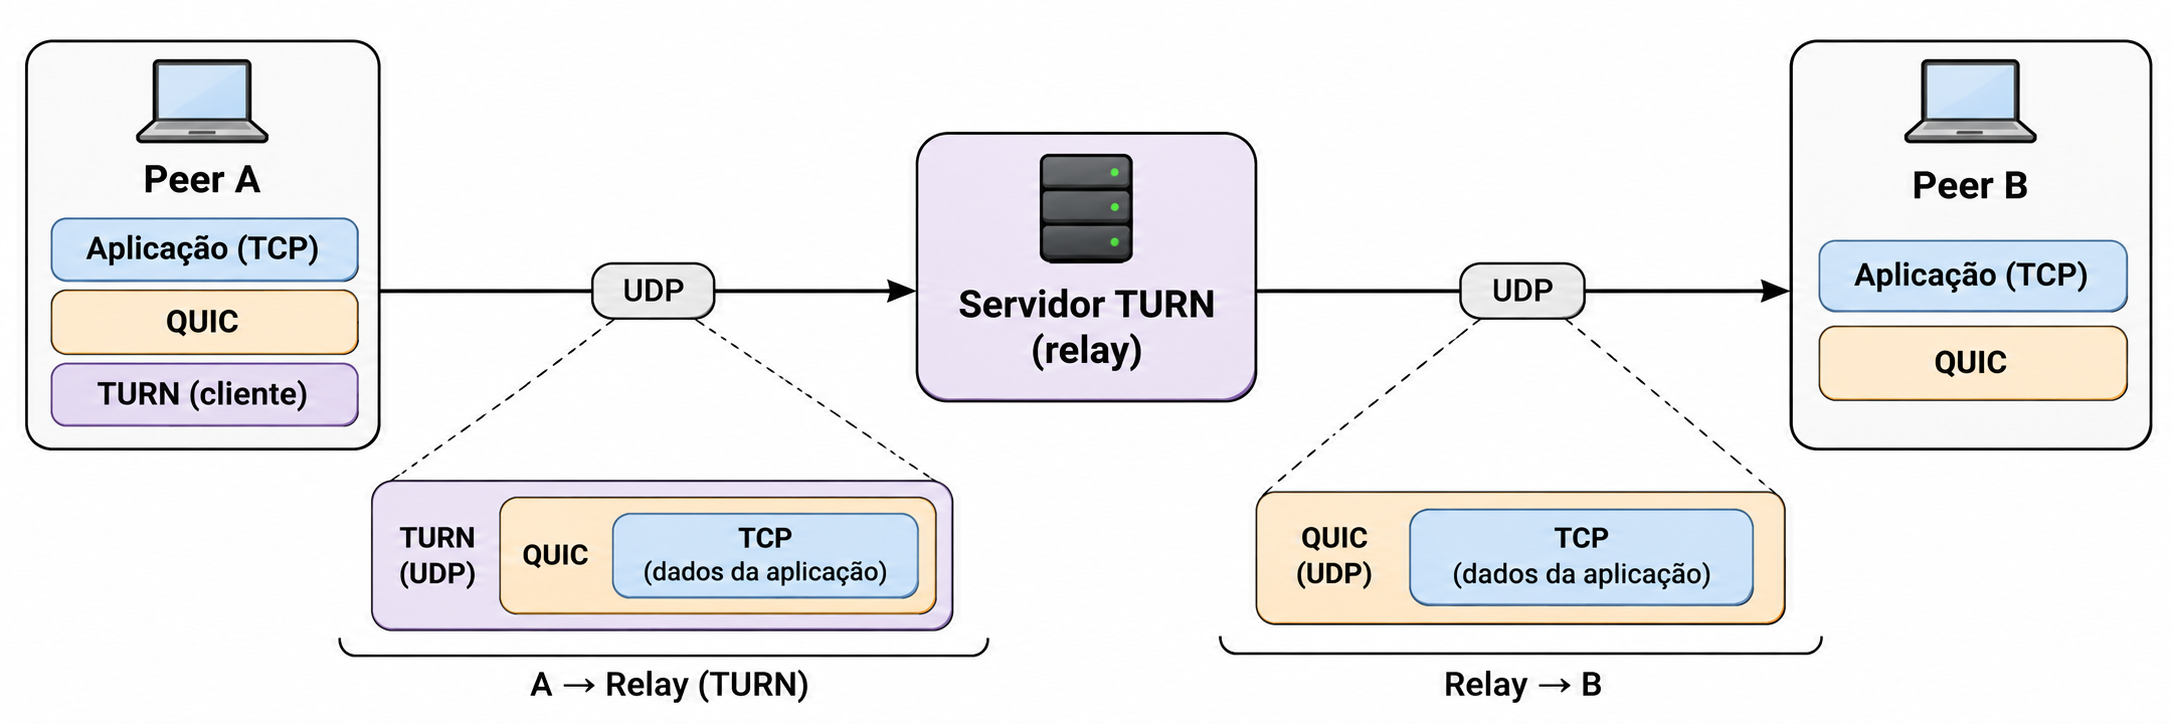
\includegraphics[width=0.8\textwidth]{fig/implementation/libnice/turn_quic_tcp_tunneling.png}
    \caption{Representação de transimssão de pacote TCP tunelados sobre QUIC sendo tunelados por TURN até o servidor \textit{relay}.}
    \label{fig:turn_quic_tcp_tunneling}
\end{figure}


Até então, chamadas POSIX eram feitas passando diretamente a \textit{socket} utilizada (\texttt{sendto}, \texttt{recvfrom}, etc.). Portanto, para a adequação e manutenção dessa mesma estrutura, foi criada uma camada fina responsável por abstrair a existência da \textit{socket} UDP, permitindo que as chamadas fossem feitas sem a necessidade de acesso direto a ela. Esta camada fina é uma interface que define um contrato a ser implementado por determinadas soluções, chamada de \texttt{udp\_transport\_t}. Isto permite que implementações específicas, como o uso da \texttt{libnice}, implementem o contrato desta interface, mantendo os detalhes de sua gerência de \textit{socket} opacos, abstraídos dos usuários desta mesma camada, que, neste caso, é a própria interface \texttt{udp\_conn} e suas respectivas implementações. Além disso, a existência desta camada permite manter a solução legada, que gerencia \textit{sockets} diretamente. Essa estrutura, se representada por um diagrama, permite a flexibilidade demonstrada na Figura~\ref{fig:udp_transport_interface}, onde a solução legada foi chamada de ``Direct UDP'' e a nova solução é a solução ICE.

\begin{figure}[ht]
    \centering
    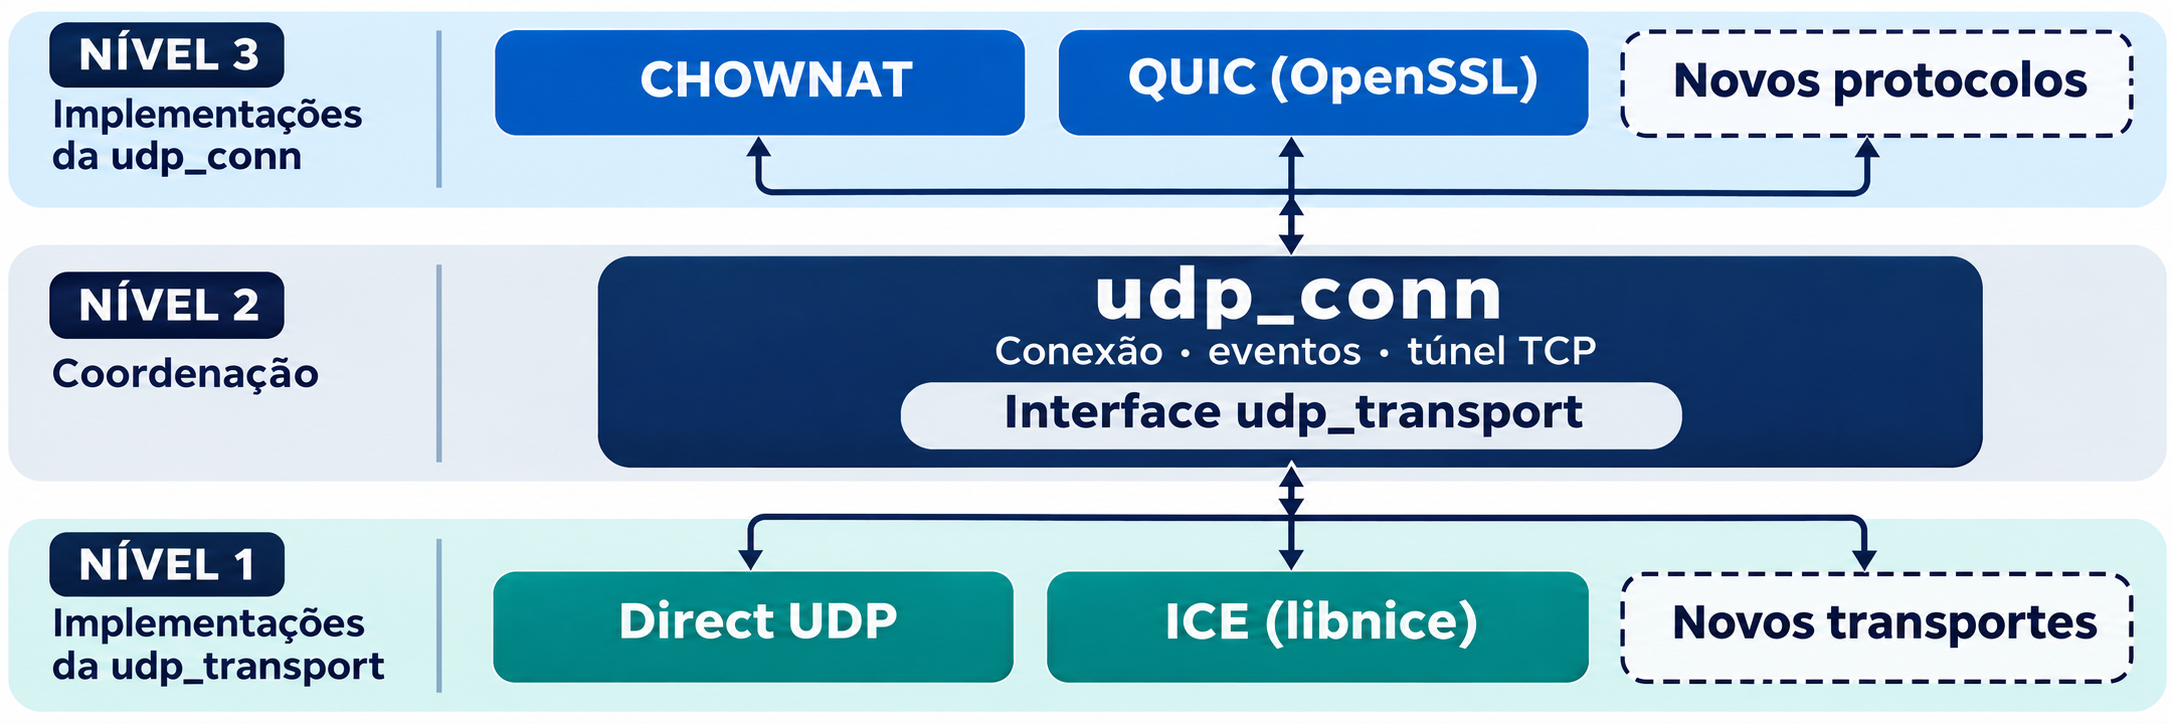
\includegraphics[width=0.8\textwidth]{fig/implementation/interface/udp_transport_flexibility.png}
    \caption{Diagrama de estrutura pós-adesão da interface \texttt{udp\_transport\_t}.}
    \label{fig:udp_transport_interface}
\end{figure}

\subsection{QUIC da OpenSSL com BIO}

Diferentemente da implementação do protocolo Chownat, em que as chamadas de manipulação de conexão e dados eram feitas através das funções da POSIX, a conexão e o transporte do protocolo QUIC da OpenSSL abstraem o uso dessas funções, fornecendo versões próprias e permitindo apenas o envio através da \textit{socket} escolhida. Portanto, não é possível simplesmente alternar sua implementação para chamar uma função de \texttt{udp\_transport}; do contrário, o \texttt{udp\_transport} precisaria conhecer a implementação QUIC, o que quebraria o contrato e inviabilizaria o isolamento da interface \texttt{udp\_transport} sem conhecimento do protocolo de transporte utilizado.

Entretanto, a OpenSSL fornece um recurso denominado BIO (\textit{Basic Input/Output}). Um BIO é uma abstração, ou pode também ser visto como outra interface, que permite abstrair o tipo de entrada e saída utilizado (arquivo, \textit{socket}, \textit{buffer}, etc.), permitindo que uma implementação específica defina um contrato próprio para o tratamento dos dados recebidos por esse BIO. Na prática, toda implementação da OpenSSL cria um BIO internamente, o que também permite que, caso outra implementação queira utilizar um contrato diferente do padrão da OpenSSL, baste implementar esse contrato. 

Esta solução resolve exatamente o problema abordado anteriormente, pois desta forma, o contrato de uma nova conexão BIO pode chamar a implementação de \texttt{udp\_transport}, abstraindo da camada acima o conhecimento sobre o protocolo de transporte utilizado. O fluxo pode ser visto na Figura~\ref{fig:openssl_quic_bio_update}.

\begin{figure}[ht]
    \centering
    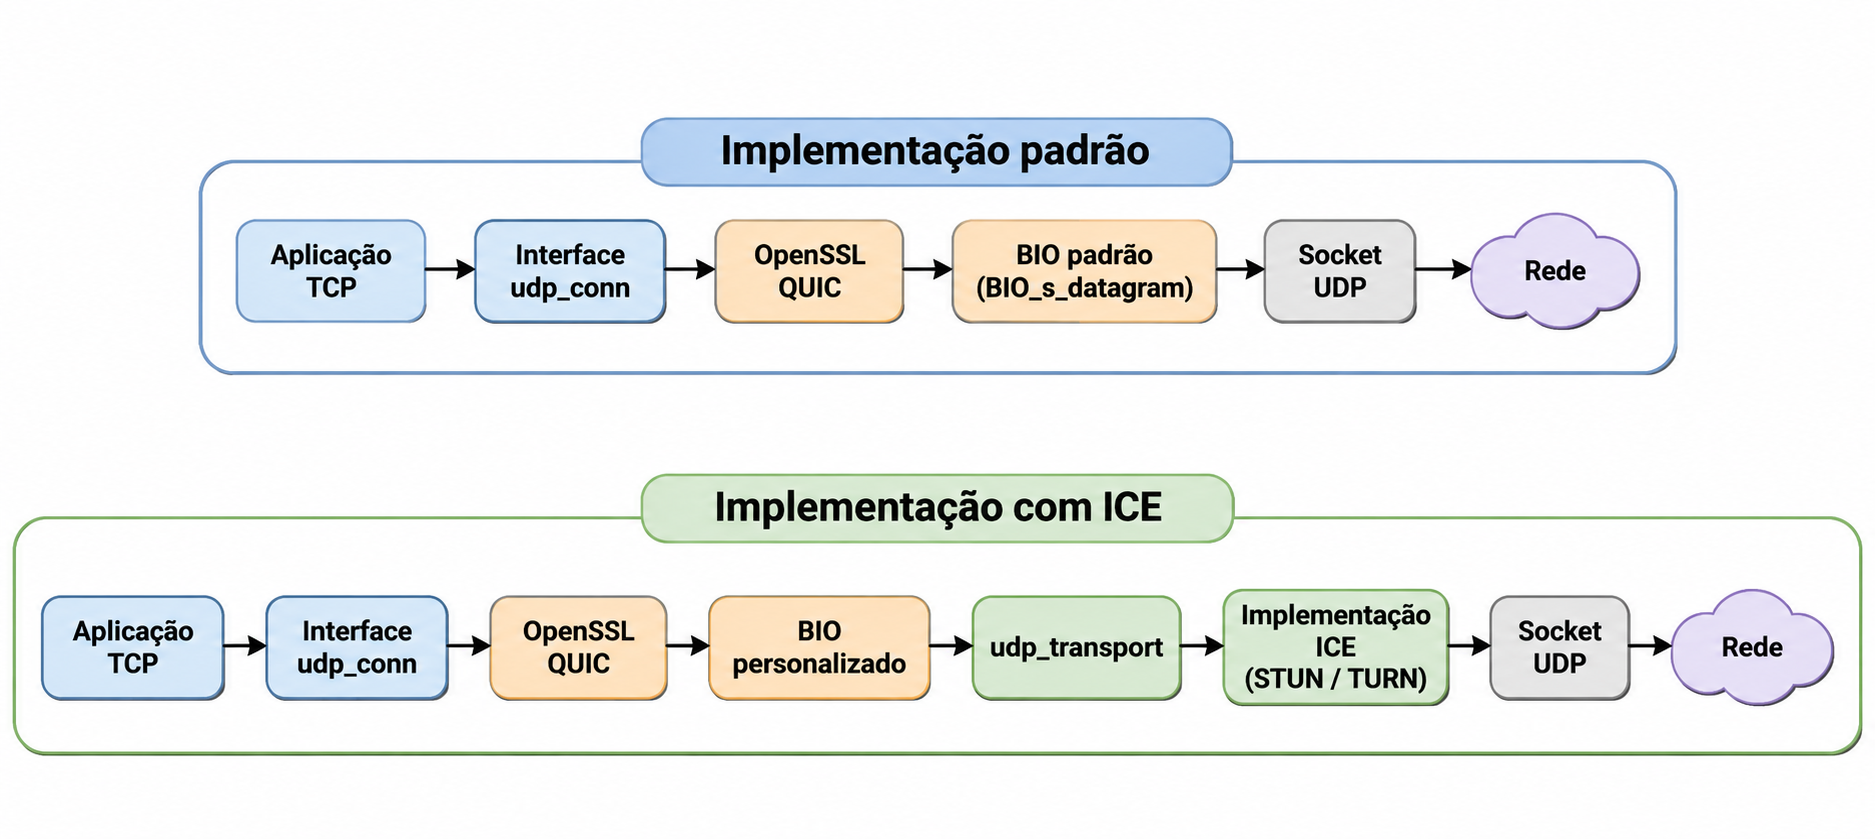
\includegraphics[width=0.9\textwidth]{fig/implementation/libnice/openssl_quic_bio_update.png}
    \caption{Diagrama de funcionamento do BIO OpenSSL juntamente com a interface \texttt{udp\_transport}.}
    \label{fig:openssl_quic_bio_update}
\end{figure}

O contrato necessário para a criação de um novo BIO, como no caso da implementação utilizada neste trabalho, é descrito por \citep{openssl_bio_meth} e exige a implementação dos seguintes métodos:

\begin{itemize}
    \item \textbf{create}: inicializar o estado específico de uma nova instância do BIO, cuja estrutura já foi alocada pela OpenSSL;
    \item \textbf{destroy}: liberar os recursos específicos da instância. A estrutura BIO em si é liberada pela OpenSSL;
    \item \textbf{ctrl}: atender comandos e consultas de controle, como \textit{flush}, configuração e obtenção de informações sobre o BIO;
    \item \textbf{sendmmsg}: enviar os datagramas fornecidos e informar quantas mensagens foram processadas;
    \item \textbf{recvmmsg}: receber datagramas nos \textit{buffers} fornecidos, preencher os tamanhos e endereços solicitados e informar quantas mensagens foram processadas.
\end{itemize}

\subsection{Funcionamento da integração da libnice}

Na arquitetura proposta, a integração da \texttt{libnice} é executada em cada \textit{gateway} e gerencia a conectividade com o \textit{gateway} remoto. Os candidatos ICE representam os caminhos disponíveis para a comunicação entre esses \textit{hosts}. Os dispositivos IoT associados ao cenário de aplicação não participam desse processo de negociação. 

Na integração da \texttt{libnice} com a interface \texttt{udp\_transport}, o usuário em nível de aplicação fica responsável apenas pela configuração desta interface, que se resume à configuração de IP/porta do servidor STUN, à configuração de IP/porta do servidor TURN e ao fornecimento de uma \textit{callback} responsável por realizar o processo de sinalização da forma que a aplicação encontrar mais adequada.

Durante as etapas de integração, grande parte das responsabilidades do protocolo ICE já são resolvidas diretamente na inicialização da interface. As configurações definidas pela aplicação são aplicadas à biblioteca, configurando cada um dos servidores. Após essa configuração, é realizada a coleta dos candidatos locais a partir dos servidores e da interface local; em seguida, é chamada a \textit{callback} definida pelo usuário para o tratamento do processo de sinalização, aguardando até que os candidatos remotos sejam recebidos. Ao recebê-los, são realizados os \textit{connectivity checks}, e, a partir da escolha dos endereços candidatos, o \textit{hole punching} é concluído, e o controle é liberado para a interface \texttt{udp\_conn}, restando como única responsabilidade pendente a gerência da conexão.

Como visto anteriormente, a \texttt{libnice} utiliza a \texttt{GLib}, uma biblioteca que fornece uma API baseada em eventos. Na implementação original da \texttt{udp\_conn}, era utilizada a chamada \texttt{select} para a gerência de múltiplas \textit{sockets}. Com a adesão da interface \texttt{udp\_transport}, essa chamada passou a ficar abstraída pela própria interface, já que ela é a responsável por gerenciar a \textit{socket} UDP. Com isso, a implementação ICE abandona o uso da chamada \texttt{select} em favor de uma variação da chamada \texttt{poll} da POSIX, também utilizada para gerenciar eventos. Dado o uso da \texttt{GLib}, a chamada utilizada é a \texttt{g\_poll}, responsável por gerenciar eventos da \texttt{GLib} e que, na prática, também utiliza \texttt{poll} internamente, ou até mesmo a própria chamada \textit{select}. Portanto, o \textit{loop} de eventos descrito anteriormente na Seção~\ref{sec:api_and_event_loop} passa a ser gerenciado internamente pela implementação de \texttt{udp\_transport}, e a gerência da conexão ICE é tratada dentro desse \textit{event loop}. Desta forma, o novo fluxo de conexão após a atualização com a biblioteca ICE se resume como visto pela Figura \ref{fig:udp_transport_connection_flow}.

\begin{figure}[ht]
    \centering
    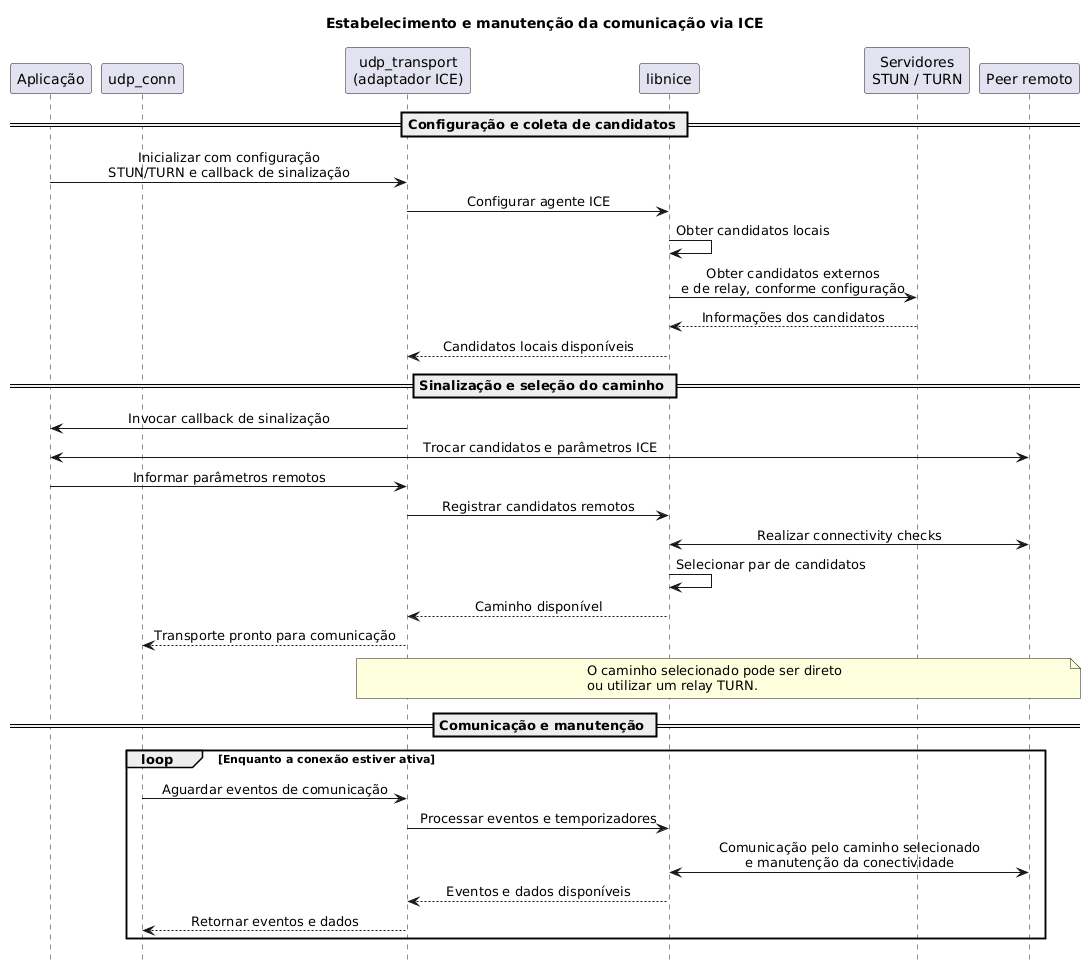
\includegraphics[width=0.8\textwidth]{fig/implementation/libnice/udp_transport_connection_flow.png}
    \caption{Diagrama de sequência do novo fluxo de conexão utilizando a biblioteca \texttt{libnice}.}
    \label{fig:udp_transport_connection_flow}
\end{figure}

\begin{comment}
    
\section{Implementação simplificada do QUIC}
\cgk{A ser feito (Implementação manual)}

\subsection{Implementação Simplificada da Conexão e Comunicação do QUIC}

\subsection{Implementação Simplificada de Connection Migration}

\subsection{Realização de Connection Migration Hole Punching}

\end{comment}

\begin{comment}
1. Transporte comum: UDP direto e ICE usam a mesma HAL. A libnice controla seus sockets, e o chamador processa eventos e timers pelo wait(), sem thread dedicada do adaptador.
2. ICE/STUN/TURN: coleta de candidatos, troca por callback de signaling, seleção do par e opção force_relay. Há testes de NAT, remapeamento de porta e TURN obrigatório.
3. CHOWNAT sobre ICE: mantém o handshake 01 → 03 → 03. A função chownat_recv_control() controla o prazo das esperas, evitando que timers ICE consumam tentativas antecipadamente.
4. QUIC sobre ICE: OpenSSL recebe datagramas por um BIO próprio ligado à HAL. Cliente e servidor usam estabelecimento e shutdown não bloqueantes com prazo. Foram separados dois streams bidirecionais, um para dados e outro para controle/keep-alive, evitando inserir bytes de controle no túnel TCP.
5. Fechamento e patch da libnice: o adaptador continua processando respostas durante o fechamento. Além disso, o build compila libnice 0.1.21 com um patch que repete a remoção TURN quando recebe 438 Stale nonce. A dependência corrigida fica estática em _deps, sem substituir a biblioteca do sistema.
\end{comment}